\chapter{Elements}
\label{c:elements}
\index{element|hyperbf}

A lattice is made up of a collection of elements --- quadrupoles,
bends, etc. This chapter discusses the various types of elements
available in \bmad.

\index{MAD}
Most element types available in \mad are provided in \bmad.
Additionally, \bmad provides a number of element types that are not
available in \mad.  A word of caution: In some cases where both \mad
and \bmad provide the same element type, there will be an overlap of
the attributes available but the two sets of attributes will not be
the same.  The list of element types known to \bmad is shown in
Table~\ref{t:particle.classes}, \ref{t:photon.classes}, and
\ref{t:control.classes}.  Table~\ref{t:particle.classes} lists the
elements suitable for use with relativistic particles,
Table~\ref{t:photon.classes} which lists the elements suitable for use
with photons, and finally Table~\ref{t:control.classes} lists the
\vn{controller} element types that can be used for parameter control
of other elements. Note that some element types are suitable for both
particle and photon use.

\begin{table}[ht]
\centering
{\tt
\begin{tabular}{|l|l||l|l|} \hline
  {\it Element}     & {\it Section}       & {\it Element}      & {\it Section}    \HH
  AB_Multipole      & \ref{s:ab.m}        &  Match             & \ref{s:match}    \HH
  BeamBeam          & \ref{s:bbi}         &  Monitor           & \ref{s:monitor}  \HH 
  Bend_Sol_Quad     & \ref{s:bsq}         &  Multipole         & \ref{s:mult}     \HH
  Branch            & \ref{s:branch}      &  Null_Ele          & \ref{s:null.ele} \HH
  Custom            & \ref{s:custom}      &  Octupole          & \ref{s:oct}      \HH
  Drift             & \ref{s:drift}       &  Patch             & \ref{s:patch}    \HH
  E_Gun             & \ref{s:e.gun}       &  Photon_Branch     & \ref{s:branch}   \HH
  Ecollimator       & \ref{s:col}         &  Pipe              & \ref{s:monitor}  \HH
  ElSeparator       & \ref{s:elsep}       &  Quadrupole        & \ref{s:quad}     \HH
  EM_Field          & \ref{s:em.field}    &  Rbend             & \ref{s:bend}     \HH
  Fiducial          & \ref{s:fiducial}    &  Rcollimator       & \ref{s:col}      \HH
  Floor_Shift       & \ref{s:floor.ele}   &  RFcavity          & \ref{s:rfcav}    \HH
  HKicker           & \ref{s:hvkicker}    &  Sbend             & \ref{s:bend}     \HH
  Hybrid            & \ref{s:hybrid}      &  Sextupole         & \ref{s:sex}      \HH
  Init_Ele          & \ref{s:init.ele}    &  Solenoid          & \ref{s:sol}      \HH
  Instrument        & \ref{s:monitor}     &  Sol_Quad          & \ref{s:sq}       \HH
  Kicker            & \ref{s:kicker}      &  Taylor            & \ref{s:tay}      \HH
  Lcavity           & \ref{s:lcav}        &  VKicker           & \ref{s:hvkicker} \HH  
  Marker            & \ref{s:mark}        &  Wiggler           & \ref{s:wiggler}  \HH
\end{tabular}
}
\caption{Table of element types suitable for use with relativistic particles.}
\label{t:particle.classes}\center
\end{table}

\begin{table}[ht]
\centering
{\tt
\begin{tabular}{|l|l||l|l|} \hline
  {\it Element}      & {\it Section}         & {\it Element}      & {\it Section}      \HH
  Branch             & \ref{s:branch}        &  Marker            & \ref{s:mark}       \HH
  Capillary          & \ref{s:capillary}     &  Match             & \ref{s:match}      \HH
  Crystal            & \ref{s:crystal}       &  Monitor           & \ref{s:monitor}    \HH 
  Custom             & \ref{s:custom}        &  Mirror            & \ref{s:mirror}     \HH
  Drift              & \ref{s:drift}         &  Multilayer_Mirror & \ref{s:multilayer} \HH
  Fiducial           & \ref{s:fiducial}      &  Patch             & \ref{s:patch}      \HH
  Floor_Shift        & \ref{s:floor.ele}     &  Photon_Branch     & \ref{s:branch}     \HH
  Init_Ele           & \ref{s:init.ele}      &  Pipe              & \ref{s:monitor}    \HH
  Instrument         & \ref{s:monitor}       &                    &                    \HH
\end{tabular}
}
\caption{Table of element types suitable for use with photons.}
\label{t:photon.classes}\center
\end{table}

\begin{table}[ht]
\centering
{\tt
\begin{tabular}{|l|l||l|l|} \hline
  {\it Element}  & {\it Section}     & {\it Element}  & {\it Section}    \HH
  Group          & \ref{s:group}     &  Overlay       & \ref{s:overlay}  \HH
  Girder         & \ref{s:girder}    &                &                  \HH
\end{tabular}
}
\caption{Table of controller elements.}
\label{t:control.classes}\center
\end{table}

%-----------------------------------------------------------------
\section{AB_Multipole}
\label{s:ab.m}
\index{ab_multipole|hyperbf}

An \vn{ab_multipole} is a thin multipole lens up to 20th order. The
basic difference between this and a \vn{multipole} (\sref{s:mult} is
the input format. See section~\sref{s:fields} for how the multipole
coefficients are defined.

General \vn{ab_multipole} Attributes are:
\begin{center}
\tt 
\begin{tabular}{|l|l||l|l|} \hline
  {\sl Attribute Class}  & \s              & {\sl Attribute Class}      & \s              \HH
  a$n$, b$n$ multipoles  & \ref{s:multip}  & Offsets \& tilt            & \ref{s:offset}  \HH
  Aperture Limits        & \ref{s:limit}   & Length                     & \ref{s:l}       \HH
  Description strings    & \ref{s:alias}   & Is_on                      & \ref{s:is.on}   \HH 
  Reference energy       & \ref{s:energy}  & Tracking \& transfer map   & \ref{c:methods} \HH
\end{tabular}
\end{center}
\toffset

For \vn{a$n$} and \vn{b$n$}, $n$ is in the range 0 through 20.

\index{x_pitch}\index{y_pitch}
The length \vn{l} is a fictitious length that is used for synchrotron
radiation computations and affects the longitudinal position of the
next element but does not affect any tracking or transfer map
calculations.  The \vn{x_pitch} and \vn{y_pitch} attributes are not
used in tracking.

Like a \mad \vn{multipole}, an \vn{ab_multipole} will affect the
reference orbit if there is a dipole component. 

Example:
\begin{example}
  abc: ab_multipole, a2 = 0.034e-2, b3 = 5.7, a11 = 5.6e6/2
\end{example}

%-----------------------------------------------------------------
\section{BeamBeam}
\label{s:bbi}
\index{beambeam|hyperbf}

A \vn{beambeam} element simulates an interaction with an opposing
(``strong'') beam traveling in the opposite direction. The strong beam
is assumed to be Gaussian in shape. In the \vn{bmad_standard}
calculation the beam--beam kick is computed using the
Bassetti--Erskine complex error function formula\cite{b:talman}

General \vn{beambeam} attributes are:
\begin{center} 
\tt
\begin{tabular}{|l|l||l|l|} \hline
  {\sl Attribute Class}  & \s              & {\sl Attribute Class}      & \s              \HH
  Aperture Limits        & \ref{s:limit}   & Offsets, pitches, \& tilt  & \ref{s:offset}  \HH
  Description strings    & \ref{s:alias}   & Is_on                      & \ref{s:is.on}   \HH 
  Reference energy       & \ref{s:energy}  & Tracking \& transfer map   & \ref{c:methods} \HH
\end{tabular}
\end{center}
\toffset

\index{sig_x}
\index{sig_y}
\index{sig_z}
\index{n_slice}
\index{charge}
\index{bbi_constant}
Attributes specific to a \vn{beambeam} element are:
\begin{example}
  sig_x   = <Real>     ! Horizontal strong beam sigma   
  sig_y   = <Real>     ! Vertical strong beam sigma
  sig_z   = <Real>     ! Strong beam length
  charge  = <Real>     ! Strong beam charge
  n_slice = <Integer>  ! Number of strong beam slices 
  bbi_constant         ! Dependent attribute (\sref{s:depend}).
\end{example}

\index{n_part!in BeamBeam element}
\vn{n_part} is the nominal number of particles of the strong
beam. \vn{n_part} is set using the \vn{parameter} command
(\sref{s:param}) and is thus common to all \vn{beambeam} elements.  To
vary the number of particles in an individual \vn{beambeam} element use the
\vn{charge} attribute. The default is \vn{charge} = -1 which indicates
that the strong beam has the opposite charge of the weak beam.

\index{x_offset}
\index{y_offset}
\vn{sig_x}, \vn{sig_y}, \vn{sig_z} are the strong beam's sigmas. 
\vn{x_offset} and \vn{y_offset} are used to offset the
\vn{BeamBeam} element. Note that in \mad the attributes used to
offset the strong beam are called \vn{xma} and \vn{yma}. Since the
offsets might not be known until run time (they, of course, depend
upon the particular orbits), often \vn{x_offset} and \vn{y_offset}
will be set by a program rather than from the lattice file.

\index{x_pitch}
\index{y_pitch}
\vn{x_pitch} and \vn{y_pitch} gives the beam--beam interaction a
crossing angle. This is the full crossing angle, not the half-angle.
See~\sref{s:beambeam.std} for details on how a \vn{beambeam} element is tracked.

The \vn{bbi_constant} is a measure of the beam--beam interaction
strength.  It is a dependent variable and is calculated from the
equation
\Begineq
  C_{bbi} = N \, m_e \, r_e / (2 \, \pi \, \gamma \, (\sigma_x + \sigma_y))
\Endeq
In the linear region, near $x = y = 0$, the 
beam--beam kick is approximately 
\begin{align}
  k_x &= -4\, \pi \, x \, C_{bbi} / \sigma_x \CRNO
  k_y &= -4\, \pi \, y \, C_{bbi} / \sigma_y 
\end{align}

The beam--beam tune shift is 
\begin{align}
  dQ_x &= C_{bbi} \, \beta_x / \sigma_x \CRNO
  dQ_y &= C_{bbi} \, \beta_y / \sigma_y \CRNO
\end{align}

Example:
\begin{example}
  bbi: beambeam, sig_x = 3e-3, sig_y = 3e-4, x_offset = 0.05
\end{example}

%-----------------------------------------------------------------
\section{Bend_Sol_Quad}
\label{s:bsq}
\index{bend_sol_quad|hyperbf}

A \vn{bend_sol_quad} is a combination bend, solenoid, and quadrupole
with the solenoid strength varying linearly with longitudinal position.
This enables the simulation of solenoid edge fields. 

General \vn{bend_sol_quad} attributes are:
\begin{center}
\tt
\begin{tabular}{|l|l||l|l|} \hline
  {\sl Attribute Class}      & \s                & {\sl Attribute Class}      & \s              \HH
  a$n$, b$n$ multipoles      & \ref{s:multip}    & Integration settings       & \ref{s:integ}   \HH
  Aperture Limits            & \ref{s:limit}     & Is_on                      & \ref{s:is.on}   \HH
  Chamber wall               & \ref{s:wall}      & Length                     & \ref{s:l}       \HH
  Description strings        & \ref{s:alias}     & Offsets, pitches, \& tilt  & \ref{s:offset}  \HH
  Field table or map         & \ref{s:em.fields} & Reference energy           & \ref{s:energy}  \HH 
  Fringe Fields              & \ref{s:fringe}    & Symplectify                & \ref{s:symp}    \HH
  Hkick \& Vkick             & \ref{s:kick}      & Tracking \& transfer map   & \ref{c:methods} \HH
\end{tabular}
\end{center}
\toffset

\index{x_quad}
\index{y_quad}
\index{quad_tilt}
\index{tilt}
\index{dks_ds}
\index{g}
\index{bend_tilt}
\index{angle}
\index{rho}
\index{k1}
\index{ks}
Attributes specific to a \vn{bend_sol_quad} element are:
\begin{example}
  g         = <Real>    ! Bend strength 1/rho
  angle     = <Real>    ! Bend angle. A settable dependent variable (\sref{s:depend})
  rho       = <Real>    ! Bend radius. A settable dependent variable (\sref{s:depend})
  bend_tilt = <Real>    ! Bend tilt angle. See \sref{s:offset}.
  k1        = <Real>    ! Quad strength.
  x_quad    = <Real>    ! Quad horizontal offset.
  y_quad    = <Real>    ! Quad vertical offset.
  quad_tilt = <Real>    ! Quad tilt. See \sref{s:offset}.
  ks        = <Real>    ! Solenoid strength.
  dks_ds    = <Real>    ! Solenoid field variation.      
  tilt      = <Real>    ! Overall tilt. See \sref{s:offset}
\end{example}

The magnetic
field is:
\begin{alignat}{1}
  \frac{q \, B_x}{P_0} &= -g_y + k_{1n} (y - y_q) - k_{1s} (x - x_q) - \frac{dks/ds}{2} \, x \CRNO
  \frac{q \, B_y}{P_0} &=  g_x + k_{1n} (x - x_q) + k_{1s} (y - y_q) - \frac{dks/ds}{2} \, y \CR
  \frac{q \, B_s}{P_0} &=  k_s + dks/ds                        \nonumber
\end{alignat}
The reference trajectory is along the solenoid centerline. The
quadrupole field is offset from the solenoid by (\vn{x_quad},
\vn{y_quad}). The quadrupole and bend have individual tilts
\vn{quad_tilt} and \vn{bend_tilt} respectively.  \vn{tilt} gives an
overall tilt. Thus the normal and skew quadrupole components $k_{1n}$,
and $k_{1s}$ are given by
\begin{example}
  k_1n = k1 * cos (2*(tilt + quad_tilt))
  k_1s = k1 * sin (2*(tilt + quad_tilt))
\end{example}
and the dipole bend components ($g_x$, $g_y$) are given by
\begin{example}
  g_x = g * cos (tilt + bend_tilt)
  g_y = g * sin (tilt + bend_tilt)
\end{example}
Dipole edge fields have not been implemented since it is not clear where
the entrance and exit faces of the bend should be and how they are aligned
with the solenoid.

To simulate a real solenoid you will need at least three
\vn{bend_sol_quad} elements: The middle element is the body of the
solenoid with the linear solenoid strength \vn{dks_ds} = 0 and the two
end elements have nonzero \vn{dks_ds} to simulate the solenoid edges.

Currently, tracking through a \vn{Bend_Sol_Quad} is via symplectic integration only.
\vn{bmad_standard} tracking is not an option since there is a possibility in
the future to implement tracking via a closed formula. 
Example:
\begin{example}
  bsq: bend_sol_quad, l = 3.7, ks = -2.3, dks_ds = 4.7, g = 1/87
\end{example}


%-----------------------------------------------------------------
\section{Bends: Rbend and Sbend}
\label{s:bend}
\index{sbend|hyperbf}
\index{rbend|hyperbf}

\vn{Rbend}s and \vn{sbend}s are dipole bends. 

General \vn{rbend} and \vn{sbend} attributes are:
\begin{center}
\tt
\begin{tabular}{|l|l||l|l|} \hline
  {\sl Attribute Class}      & \s                & {\sl Attribute Class}      & \s              \HH
  a$n$, b$n$ multipoles      & \ref{s:multip}    & Integration settings       & \ref{s:integ}   \HH
  Aperture Limits            & \ref{s:limit}     & Is_on                      & \ref{s:is.on}   \HH
  Chamber wall               & \ref{s:wall}      & Length                     & \ref{s:l}       \HH
  Description strings        & \ref{s:alias}     & Offsets, pitches, \& tilt  & \ref{s:offset}  \HH
  Field table or map         & \ref{s:em.fields} & Reference energy           & \ref{s:energy}  \HH 
  Fringe Fields              & \ref{s:fringe}    & Symplectify                & \ref{s:symp}    \HH
  Hkick \& Vkick             & \ref{s:kick}      & Tracking \& transfer map   & \ref{c:methods} \HH
\end{tabular}
\end{center}
\toffset

\index{g}\index{b_field}\index{g_err}\index{b_field_err}\index{angle}
\index{l_chord}\index{angle}\index{h1}\index{h2}
\index{e1}\index{e2}\index{fint}\index{fintx}\index{l_arc}
\index{hgap}\index{hgapx}\index{roll}\index{k1}
Attributes specific to \vn{rbend} and \vn{sbend} elements are:
\begin{example}
  g           = <Real>     ! Design bend strength (= 1/rho).
  g_err       = <Real>     ! Bend strength error (\sref{s:depend}).
  b_field     = <Real>     ! Design field strength (= P_0 g / q) (\sref{s:depend}).
  b_field_err = <Real>     ! Field strength error (\sref{s:depend}).
  angle       = <Real>     ! Design bend angle. A settable dependent variable (\sref{s:depend}).
  rho         = <Real>     ! Design bend radius. A settable dependent variable (\sref{s:depend}).
  e1, e2      = <Real>     ! Face angles.
  exact_bend  = <Logical>  ! Use better edge tracking.
  fint, fintx = <Real>     ! Face field integrals.
  hgap, hgapx = <Real>     ! Pole half gap.
  h1, h2      = <Real>     ! Face curvature.
  roll        = <Real>     ! See \ref{s:offset}.
  k1          = <Real>     ! Quadrupole strength.
  k2          = <Real>     ! Sextupole strength (\sref{s:depend}).
  b1_gradient = <Real>     ! Quadrupole field strength (\sref{s:depend}).
  b2_gradient = <Real>     ! Sextupole field strength (\sref{s:depend}).
  n_ref_pass  = <Int>      ! Multipass reference turn (\sref{s:multipass}).
  l_arc       = <Real>     ! Arc length. For \vn{rbend}s only. 
  l_chord                  ! Chord length. Dependent attribute. See \sref{s:l}.
  ptc_field_geometry 
              = <Switch>   ! 
\end{example}

\index{l}
The difference between \vn{rbend} and \vn{sbend} elements
is the way the \vn{l}, \vn{e1}, and \vn{e2} attributes are interpreted.
To ease the bookkeeping burden, after reading in a lattice, \bmad will
internally convert all \vn{rbend}s into \vn{sbend}s. 
This is done using the following transformation on \vn{rbend}s:
\begin{example}
  l_chord(internal) = l(input)
  l(internal) = 2 * asin(l_chord * g / 2) / g
  e1(internal) = e1(input) + theta / 2
  e2(internal) = e2(input) + theta / 2
\end{example}

\begin{figure}[tb]
  \centering
  \subfigure[rbend]
  {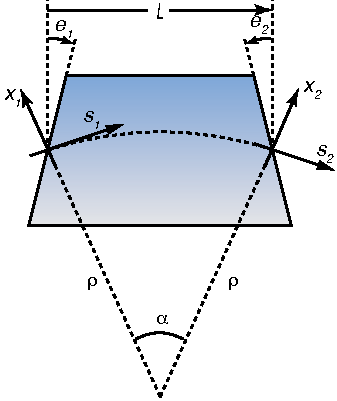
\includegraphics{rbend-coords.pdf}}
  \hspace{1cm}
  \subfigure[sbend]
  {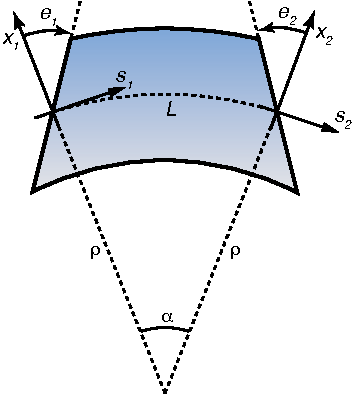
\includegraphics{sbend-coords.pdf}}
  \caption[Coordinate systems for (a) \vn{rbend}\ and (b) \vn{sbend}\ elements.]
{Coordinate systems for (a) \vn{rbend} and (b) \vn{sbend} elements.
For the bends drawn as viewed from ``above'' (viewed from positive $y$),
\vn{g}, \vn{angle}, \vn{rho}, \vn{e1} and \vn{e2} are all positive.}
  \label{f:bend}
\end{figure}

  \begin{description}
  \index{l}\index{l_chord}\index{l_arc}
  \item[l, l_chord]  \Newline
For compatibility with MAD, for an \vn{rbend}, \vn{l} is the chord
length and not the arc length as it is for an \vn{sbend}.  However,
after reading in a lattice, \bmad will internally convert all
\vn{rbend}s into \vn{sbend}s, additionally, the \vn{l_chord} attribute
will be set to the input \vn{l}, and \vn{l} will be set to the true
path length (see above). Alternatively, instead of setting \vn{l}, the
\vn{l_arc} attribute can be set to the true arc length.
  \index{h1}\index{h2}
  \item[h1, h2] \Newline
The attributes \vn{h1} and \vn{h2} are the curvature of the entrance
and exit pole faces. They are present for compatibility with MAD but
are not yet implemented in terms of tracking and other calculations.
  \index{e1}\index{e2}
  \item[e1, e2] \Newline
The rotation angle of the entrance pole face is \vn{e1} and at the
exit face it is \vn{e2}. Zero \vn{e1} and \vn{e2} for an \vn{rbend}
gives a rectangular magnet  (\fig{f:bend}a). Zero \vn{e1} and \vn{e2}
for an \vn{sbend} gives a wedge shaped magnet (\fig{f:bend}b).
An \vn{sbend} with an \vn{e1} = \vn{e2} = \vn{angle}/2 is equivalent 
to an \vn{rbend} with \vn{e1} = \vn{e2} = 0 (see above).
This formula holds for both positive and negative angles.
  \index{angle}
  \item[angle] \Newline
The total design bend angle. A positive \vn{angle} represents a
bend towards negative $x$ values (see \fig{f:local.coords}).
  \index{k1}\index{b1_gradient}
  \item[k1, b1_gradient] \Newline
The normalized and unnormalized quadrupole strength.
  \index{k2}\index{b2_gradient}
  \item[k2, b2_gradient] \Newline
The normalized and unnormalized sextupole strength. 
  \index{g}\index{rho}\index{g_err}
  \item[g, g_err, rho] \Newline
The design bending radius which determines the reference coordinate
system is \vn{rho} (see \sref{s:ref}). \vn{g} = 1/\vn{rho} is
the curvature function and is proportional to the design dipole
magnetic field. The true field strength is given by
\vn{g}~+~\vn{g_err} so changing \vn{g_err} leaves the design orbit
unchanged but varies a particle's orbit.
  \index{fint}\index{fintx}\index{hgapx}\index{hgapx}
  \item[fint, fintx, \Newline hgap, hgapx] \Newline
The field integrals for the entrance and
exit pole faces are give by \vn{fint} and \vn{fintx} respectively
\Begineq
  F_{int} = \int_{pole} \! \! ds \, \frac{B_y(s) (B_{y0} - B_y(s))}
  {2 H_{gap} B_{y0}^2}
\Endeq
with a similar equation for \vn{fintx}. In the equation $B_{y0}$ is
the field in the interior of the dipole and $H_{gap}$ is the pole half
gap.  The parameters \vn{hgap} and \vn{hgapx} are the half gaps at the
entrance and exit faces. If \vn{fint} or \vn{fintx} is given without a
value then a value of 0.5 is used. If \vn{fint} or \vn{fintx} is not
present, the default value of 0 is used. Note: \mad does not have the
\vn{fintx} and \vn{hgapx} attributes. \mad just assumes that the
values are the same for the entrance and exit faces. For compatibility
with \mad, if \vn{fint} is given but \vn{fintx} is not, then
\vn{fintx} is set equal to \vn{fint}. Similarly, \vn{hgapx} will be
set to \vn{hgap} if \vn{hgapx} is not given.

\index{Enge function}
\vn{fint} and \vn{hgap} can be related to the Enge function which is sometimes
used to model the fringe field. The Enge function is of the form
\Begineq
  B_y(s) = \frac{B_{y0}}{1 + \exp[P(s)]}
\Endeq
where
\Begineq
  P(s) = C_0 + C_1 \, s + C_2 \, s^2 + C_3 \, s^3 + \, \ldots
\Endeq
The $C_0$ term simply shifts where the edge of the bend is. If all the $C_n$
are zero except for $C_0$ and $C_1$ then 
\Begineq
  C_1 = \frac{1}{2 \,H_{gap} \, F_{int}}
\Endeq
  \index{tilt}
  \item[tilt] \Newline
The roll angle about the longitudinal axis at the entrance face of the
bend is given by \vn{tilt}.  \vn{tilt} = 0 bends the reference
trajectory in the $-x$ direction.  If the \vn{tilt} attribute is given
without any value then the value $\pi/2$ will be used. This makes for
a \vn{downward} pointing vertical bend. See \fig{f:tilt.bend}.
  \end{description}

The attributes \vn{g}, \vn{angle}, and \vn{l} are mutually dependent. If any two are
specified for an element \bmad will calculate the appropriate value
for the third.  After reading in a lattice, \vn{angle} is considered a
dependent variable (\sref{s:depend}).

Since internally all \vn{rbend}s are converted to \vn{sbend}s, if one wants to
vary the \vn{g} attribute of a bend and still keep the bend rectangular, an
overlay (\sref{s:overlay}) can be constructed to maintain the proper face angles.
For example:
\begin{example}
  l_ch = 0.54
  g_in = 1.52
  l_coef = asin(l_ch * g_in / 2) / g_in
  my_bend: rbend, l = l_ch, g = g_in
  my_overlay: overlay = \{my_bend, my_bend[e1]:l_coef, my_bend[e2]:l_coef\}, g = g_in
\end{example}
Notice that \vn{l_coef} is just \vn{arc_length/2}.

The \vn{n_ref_pass} attribute are only used
when a bend is part of a \vn{multipass} line and is used to set the
reference geometry of the bend. See section~\sref{s:multipass} for
more details.

In the local coordinate system (\sref{s:ref}), looking from ``above''
(bend viewed from positive $y$), and with \vn{tilt} = 0, a positive
\vn{angle} represents a particle rotating clockwise. In this
case. \vn{g} will also be positive. For counterclockwise rotation,
both \vn{angle} and \vn{g} will be negative but the length \vn{l} is
always positive. Also, looking from above, a positive \vn{e1}
represents a clockwise rotation of the entrance face and a positive
\vn{e2} represents a counterclockwise rotation of the exit face. This
is true irregardless of the sign of \vn{angle} and \vn{g}. Also it is
always the case that the pole faces will be parallel when
\begin{example}
  e1 + e2 = angle
\end{example}

\begin{figure}[tb]
  \centering
  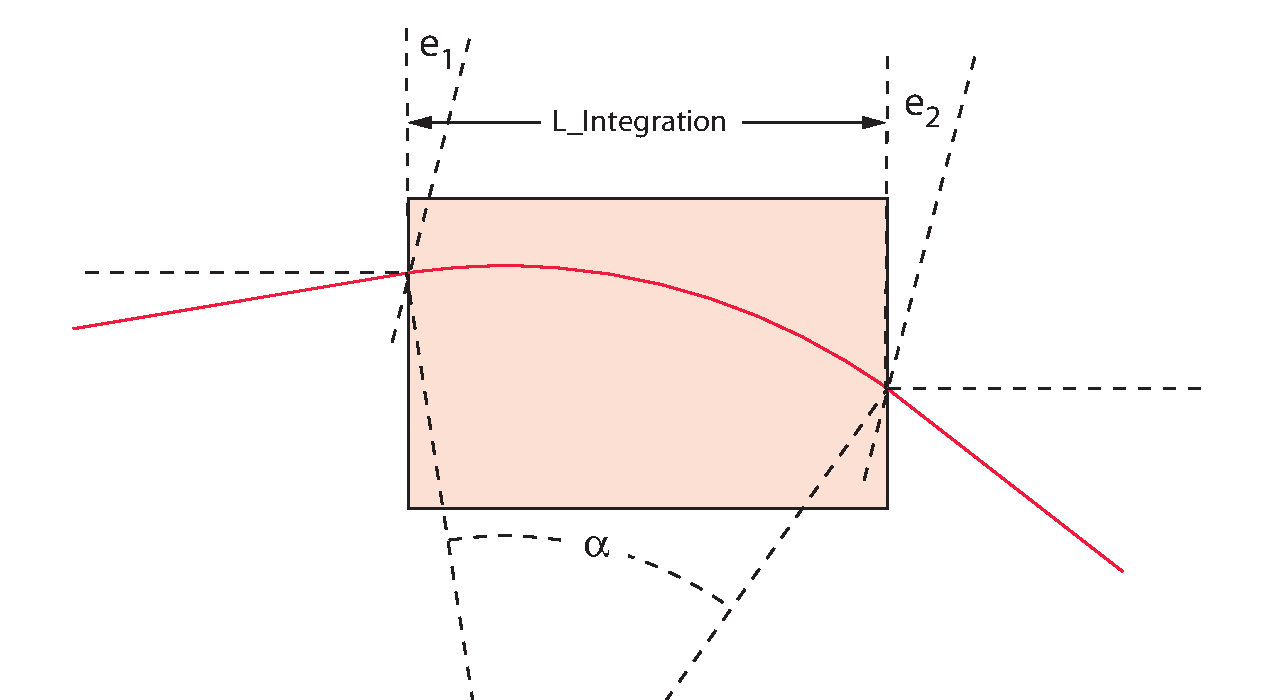
\includegraphics[width=5in]{true-rbend.pdf}
  \caption[True Rbend coordinates]{Coordinate system when \vn{ptc_field_geometry}
is set to \vn{true_rbend}.}
  \label{f:true.rbend}
\end{figure}

Example bend specification:
\begin{example}
  b03w: sbend, l = 0.6, k1 = 0.003, fint  ! gives fint = fintx = 0.5
\end{example}


\vn{ptc_field_geometry} determines how PTC integrates through a bend
if PTC is being used for tracking. Possible values for
\vn{ptc_field_geometry} are:
\begin{example}
  sector      ! Default
  straight
  true_rbend  ! Only valid for rbend elements
\end{example}
For \vn{sector} tracking, the tracking coordinate reference frame is
with respect to the arc of the reference trajectory. For \vn{straight}
tracking the tracking coordinate reference frame is with respect to the
chord line. For a bend where the number of integration steps is large
enough, and where there are no other fields besides the basic dipole
field, the results are the same.  When there are quadrupole or higher
order fields, the fields are expanded about the tracking reference
frame. Since Maxwell's equations must be satisfied, the higher order
fields will differ when tracking with \vn{sector} vs \vn{straight} the
difference in the fields will scale with the inverse of the bending
radius \vn{1/rho}. The above discussion is true for
\vn{ptc_exact_model} set to True, for \vn{ptc_exact_model} set to
False, a simplified sector tracking model is used in all cases.

The \vn{true_rbend} tracking of \vn{ptc_field_geometry} is used only
with \vn{rbend} elements and the entrance and exit faces must be parallel
as shown in \fig{f:true.rbend}. That is
\begin{example}
  e1 + e2 = 0
\end{example}
In this case, the tracking geometry is parallel, to the bend face as
shown in the figure. This can be an advantage in some situations but
Etienne discourages use of \vn{true_rbend} due to complications of how
to handle the reference frames in particular when you have more than
one of them in a row.

%-----------------------------------------------------------------
\section{Branch and Photon_Branch}
\label{s:branch}
\index{branch|hyperbf}
\index{photon_branch|hyperbf}

A \vn{branch} or \vn{photon_branch} element marks the start of an
alternative line for the beam. The only difference between \vn{branch}
and \vn{photon_branch} is that the default particle type for a
\vn{branch} is the same particle type in use at where the branching
occurs. The default particle type for a \vn{photon_branch} element is
a photon.

Collectively \vn{branch} and \vn{photon_branch} elements can be called
branching elements.

General \vn{branch} and \vn{photon_branch} attributes are:
\begin{center}
\tt
\begin{tabular}{|l|l||l|l|} \hline
  {\sl Attribute Class}  & \s              & {\sl Attribute Class}      & \s              \HH
  Description strings    & \ref{s:alias}   & Offsets, pitches, \& tilt  & \ref{s:offset}  \HH
  Reference energy       & \ref{s:energy}  & Tracking \& transfer map   & \ref{c:methods} \HH
  Aperture Limits        & \ref{s:limit}   & Length                     & \ref{s:l}       \HH
                         &                 & Is_on                      & \ref{s:is.on}   \HH 
\end{tabular}
\end{center}
\toffset

Attributes specific to \vn{branch} and \vn{photon_branch} elements are:
\begin{example}
  direction    = <+/- 1>      ! Direction of branch.
  to_line      = <LineName>   ! What line to branch to.
  to_element   = <ElementID>  ! What element to in the line to attach to.
  new_branch   = <T/F>        ! Make a new branch from the to_line? Default = True.
\end{example}

Branch lines can themselves have branching elements. A branch line
always starts out tangential to the line it is branching from. The
\vn{direction} attribute of the branch element indicates whether the
branch line is outgoing in the forward direction (\vn{direction} = +1)
or incoming (\vn{direction} = -1). A \vn{patch} element
(\sref{s:patch}) can be used at the beginning of a branch line to
reorient the reference orbit as needed.

The offset, pitch, and tilt attributes of a branching element can be
used to offset the reference orbit of the element being branched
to. This is analogous to using a rigid \vn{patch} element
(\sref{s:patch}) to modify the reference orbit within a branch. See
Section~\sref{s:patch} for more details.  Example:
\begin{example}
  from_line: line = (... A, PB, B, ...)  ! Line containing a branch
  x_line: line = (X1, X2, ...)           ! Line branched to
  pb: photon_branch, x_offset = 0.01, to_line = x_line
  use, from_line
\end{example}
In this example, a photon generated at the branch element \vn{PB} with
$x = 0$ with respect to the \vn{from_line} reference orbit through
\vn{PB} will, when transferred to the \vn{x_line}, have an initial
value for $x$ of $-0.01$ due to the setting of the \vn{x_offset} 
parameter of \vn{PB}.

Branching elements have zero length and within a lattice branch, a
branching element acts like a \vn{marker}. Using the above example, a
particle that is being tracked down the \vn{from_line} will have the
same phase space coordinates at the end of element \vn{PB} as it had
at the end of element \vn{A}. That is, the offset, pitches, and tilt
attributes of a branching element only affect particles that are
transferred to the \vn{to_line} when arriving at the branching element.
particles that remain on the original lattice branch will be
unaffected by any offset, pitches or tilt settings. 

If the branch line is to transport particles different from the
originating line the particle type and the beginning reference energy
must be set for that line using line parameter statements
(\sref{s:beginning}). This is useful, for example, for a photon branch
that is branching from a storage ring where the photon energy is not
simply related to the particle energy. 

Example showing an injection line branching to a ring branching to two
x-ray lines:
\begin{example}
  inj: line = (..., ring_br, ...)            ! Define the injection line
  use, inj                                   ! Injection line is the root
  ring_br: branch, to_line = ring, 
          geometry = closed                  ! Branch to the ring
  ring: line = (..., x_br, ..., x_br, ...)   ! Define the ring
  x_br: photon_branch, to_line = x_line 
  x_line: line = (...)                       ! Define the x-ray line
  x_line[E_tot] = 1e3
\end{example}

The \vn{new_branch} attribute is, by default, \vn{True} which means
that the lattice branch created out of the \vn{to_line} line is distinct
from other lattice branches of the same name. Thus, in the above example,
the two lattice branches made from the \vn{x_line}
will be distinct. If \vn{new_branch} is set to \vn{False}, a new lattice
branch will not be created if a lattice branch created from the same
line already exists. This is useful, for example, when a chicane line
branches off from the main line and then branches back to it.

The root branches of a lattice are defined by the \vn{use}
(\sref{s:use}) statement. To further define such things as dump lines,
x-ray beam lines, transfer lines, etc., that branch off from a root
branch, a branching element is used.  \vn{Branch} elements can define
where the particle beam can branch off, say to a beam
dump. \vn{photon_branch} elements can define the source point for
X-ray beams.  Example:
\begin{example}
  erl: line = (..., dump, ...)               ! Define the root branch 
  use, erl
  dump: branch, to = d_line                  ! Define the branch point

  d_line: line = (..., q3d, ...)             ! Define the branch line
\end{example}
The difference between a \vn{branch} element and a \vn{photon_branch}
element is that for a \vn{branch} element the default particle for the
branch is the same as the line that the branch branches off from. The
default particle of the branch from a \vn{photon_branch} element is a
\vn{photon}. The actual particle associated with a branch can be set
by setting the \vn{particle} attribute of the branching element
(\sref{s:branch}).

Like the root branch \bmad always automatically creates an element
with \vn{element index} 0 at the beginning of each branch called
\vn{beginning}. The longitudinal \vn{s} position of an element in a
branch is determined by the distance from the beginning of the branch.

Branch parameters, like whether the branch is open
(``open'') or closed (``closed''), can be set
by setting the appropriate attribute of the \vn{branch} or
\vn{photon_branch} element used to orient the branch.
See \sref{s:branch} for more details.

Branches are named after the branching element name. In the above
example, the branch line would be named \vn{DUMP}. The root branch, by
default, is called after the name in the \vn{use} statement
(\sref{s:use}).

For branch lines (\sref{s:branch}), the ``branch
qualified'' name of an element is of the form
\begin{example}
  branch_name>>element_name
\end{example}
where \vn{branch_name} is the name of the branch and \vn{element_name} is the
``regular'' name of the element. Example:
\begin{example}
  root>>q10w
  xline>>cryst3
\end{example}
When parsing a lattice file, branches are not formed until the lattice
is expanded (\sref{s:expand}). Therefore an \vn{expand_lattice}
statement is required before branch qualified names can be used in
statements.  See \sref{s:ele.names} for more details.

%-----------------------------------------------------------------
\section{Capillary}
\label{s:capillary}
\index{capillary|hyperbf}

A \vn{capillary} element is a glass tube that is used to focus x-ray
beams.

General \vn{capillary} attributes are:
\begin{center}
\tt
\begin{tabular}{|l|l||l|l|} \hline
  {\sl Attribute Class}  & \s              & {\sl Attribute Class}      & \s              \HH
  Description strings    & \ref{s:alias}   & Offsets, Pitches \& Tilt   & \ref{s:offset}  \HH
  Reference energy       & \ref{s:energy}  & Tracking \& transfer map   & \ref{c:methods} \HH
  Aperture Limits        & \ref{s:limit}   & Is_on                      & \ref{s:is.on}   \HH 
  Capillary Wall         & \ref{s:wall}    &                            &                 \HH
\end{tabular}
\end{center}
\toffset

\index{critical_angle_factor|hyperbf}
Attributes specific to a \vn{capillary} element are:
\begin{example}
  critical_angle_factor = <Real>    ! Critical angle * Energy (rad * eV)
\end{example}
The critical angle above which photons striking the capillary surface are
refracted into the capillary material scales as 1/Energy. The
constant of critical angle * energy is given by the \vn{critical_angle_factor}.

The inside wall of a capillary is defined using the same syntax used
to define the chamber wall for other elements (\sref{s:wall}).

%-----------------------------------------------------------------
\section{Collimators: Ecollimator and Rcollimator} 
\label{s:col}
\index{ecollimator|hyperbf}
\index{rcollimator|hyperbf}

An \vn{ecollimator} is a drift with elliptic collimation. An
\vn{rcollimator} is a drift with rectangular collimation.

General \vn{ecollimator} and \vn{rcollimator} attributes are:
\begin{center}
\tt
\begin{tabular}{|l|l||l|l|} \hline
  {\sl Attribute Class}  & \s              & {\sl Attribute Class}      & \s              \HH
  Description strings    & \ref{s:alias}   & Offsets, Pitches \& Tilt   & \ref{s:offset}  \HH
  Reference energy       & \ref{s:energy}  & Tracking \& transfer map   & \ref{c:methods} \HH
  Aperture Limits        & \ref{s:limit}   & Length                     & \ref{s:l}       \HH
  Symplectify            & \ref{s:symp}    & Integration settings       & \ref{s:integ}   \HH
  Hkick \& Vkick         & \ref{s:kick}    & Chamber wall               & \ref{s:wall}    \HH
\end{tabular}
\end{center}
\toffset

Note: Collimators are the exception to the rule that the aperture is
independent of any \vn{tilt}s. See \sref{s:limit} for more
details. Example:
\begin{example}
  d21: ecollimator, l = 4.5, x_limit = 0.09/2, y_limit = 0.05/2
\end{example}

%-----------------------------------------------------------------
\section{Crystal}
\label{s:crystal}
\index{crystal|hyperbf}

\begin{figure}[tb]
  \centering
  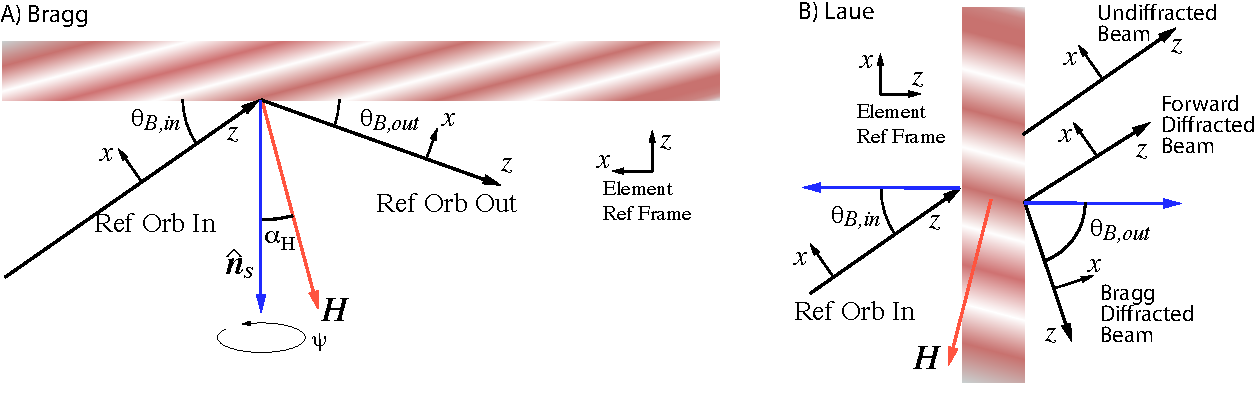
\includegraphics[width=5in]{crystal-ele.pdf}
  \caption[Crystal element geometry.]
{Crystal element geometry.  A) Geometry for Bragg diffraction. The
geometry shown is for \vn{tilt} = 0 (reference trajectory in the
$x$-$z$ plane). The angle $\alpha_H$ (\vn{alpha_angle}) is the angle
of the $\bfH$ vector with respect to the surface normal $\bfhat
n$. For $\psi$ (\vn{psi_angle}) zero, the incoming reference orbit,
the outgoing reference orbit, $\bfhat n$, and $\bfH$ are all
coplanar. The element reference coordinates where $\bfhat x$ is
parallel to the surface normal establishes the coordinates for
specifying a rotation of $\bfH$ around the surface normal and
specifying a curvature of the surface. B) Geometry for Laue
diffraction. In this case there are three outgoing beams: The Bragg
diffracted beam, the forward diffracted beam, and the undiffracted
beam.}
  \label{f:crystal}
\end{figure}

A \vn{crystal} element represents a crystal used for photon diffraction.

General \vn{crystal} attributes are:
\begin{center}
\tt
\begin{tabular}{|l|l||l|l|} \hline
  {\sl Attribute Class}  & \s              & {\sl Attribute Class}      & \s              \HH
  Description strings    & \ref{s:alias}   & Offsets, Pitches \& Tilt   & \ref{s:offset}  \HH
  Reference energy       & \ref{s:energy}  & Tracking \& transfer map   & \ref{c:methods} \HH
  Aperture Limits        & \ref{s:limit}   & Symplectify                & \ref{s:symp}    \HH
  Chamber Wall           & \ref{s:wall}    & Surface Curvature          & \ref{s:s.curve} \HH
\end{tabular}
\end{center}
\toffset

\index{psi_angle}
\index{b_param}\index{bragg_angle}\index{crystal_type}
\index{tilt_err}\index{g_graze}
\index{follow_diffracted_beam}\index{thickness}
Attributes specific to a \vn{crystal} element are:
\begin{example}
  b_param            = <Real>       ! b parameter
  crystal_type       = <String>     ! Crystal material and reflection plane.
  psi_angle          = <Real>       ! Rotation of H-vector about the surface normal.
  tilt_err           = <Real>       ! Error in the tilt angle.
  thickness          = <Real>       ! Thickness of crystal for Laue diffraction.
  ref_orbit_follows  = <which_beam> ! Reference orbit aligned with what outgoing beam?
\end{example}

\index{graze_angle_in}\index{graze_angle_out}\index{alpha_angle}
\index{tilt_corr}\index{d_spacing}\index{v_unitcell}\index{f0_re}
\index{f0_im}\index{fh_re}\index{fh_im}\index{ref_wave_length}
\index{c2_curve_tot}\index{c3_curve_tot}\index{c4_curve_tot}
Dependent variables (\sref{s:depend}) specific to a \vn{crystal} element are:
\begin{example}
  alpha_angle      ! Angle of H-vector with respect to the surface normal.
  bragg_angle      ! Nominal Bragg angle at the reference wave length. 
  d_spacing        ! Lattice plane spacing. 
  f0_re            ! Real part of f0
  f0_im            ! Imaginary part of f0
  fh_re            ! Real part of fh
  fh_im            ! Imaginary part of fh
  graze_angle_in   ! Angle between incoming beam and mirror surface.
  graze_angle_out  ! Angle between outgoing beam and mirror surface.
  ref_wavelength   ! Reference wavelength
  ref_cap_gamma    ! \(\Gamma\) at the reference wavelength.
  tilt_corr        ! Tilt correction due to a finite psi_angle.
  v_unitcell       ! Unit cell volume. 
\end{example}

The \vn{crystal_type} attribute defines the crystal material and
diffraction lattice plane. The syntax is \vn{"ZZZ(ijk)"} where \vn{ZZZ}
is the atomic formula for the material and \vn{ijk} are the Miller
indices for the diffraction plane. For example,
\begin{example}
  b_cryst1: crystal, crystal_type = "Si(111)", b_param = -1, ...
\end{example}
The atomic formula is case sensitive so, for example, \vn{"SI(111)"}
is not acceptable.  Given the \vn{crystal_type}, the spacing between
lattice planes (\vn{d_spacing}), the unit cell volume
(\vn{v_unitcell}), and the structure factor\cite{b:batterman} values
\vn{f0_re}, and \vn{f0_im}, can be computed. And once the reference
photon energy (\sref{s:energy}), is established, the structure factors
\vn{fh_re}, \vn{fh_im} can be evaluated.

The \vn{b_param} is the standard asymmetry factor
\Begineq
  b = \frac{\sin(\alpha_H + \theta_B)}{\sin(\alpha_H - \theta_B)} 
\Endeq
where $\theta_B$ is the Bragg angle (\vn{bragg_angle}) 
\Begineq
  \theta_B = \sin^{-1} \left( \frac{\lambda}{2 \, d} \right)
\Endeq
and $\alpha_H$ (\vn{alpha_angle}) is the angle of the reciprocal
lattice $\bfH$ vector with respect to the surface normal as shown in
\fig{f:crystal}A.  If \vn{b_param} is set to -1 then there is
Bragg reflection and \vn{alpha_H} is zero. If \vn{b_param} is set to 1
then there is Laue diffraction again with \vn{alpha_H} zero. With the
orientation shown in \fig{f:crystal}A, \vn{alpha_H} is positive.

The \vn{thickness} parameter is used with Laue diffraction only.

The \vn{ref_orbit_follows} parameter sets how the outgoing reference
orbit is constructed. This is only relevant with Laue diffraction.
The possible settings of this parameter are:
\begin{example}
  brag_diffracted
  forward_diffracted
  undiffracted
\end{example}
The geometry of this situation is shown in \fig{f:crystal}B.

If \vn{psi_angle} is zero, the incoming reference orbit, the outgoing
reference orbit, $\bfhat n$ and $\bfH$ are all coplanar. A non-zero
\vn{psi_angle} Rotates the $\bfH$ vector around the $+\bfhat x$ axis
of the \vn{Element Reference Frame} (See \fig{f:crystal}A).

To keep the outgoing reference trajectory independent of the value of
\vn{psi_angle}, the crystal will be automatically tilted by the
appropriate ``tilt correction'' \vn{tilt_corr}. The calculation of
\vn{tilt_corr} is outlined in \sref{ss:crystal.trans}. \vn{tilt_corr}
will be zero if \vn{psi_angle} is zero. Thus, for the reference orbit
calculation, the total tilt of the crystal is \vn{tilt} +
\vn{tilt_corr}.

The reference trajectory for a Bragg \vn{crystal} is that of a zero
length bend (\sref{s:mirror.coords}) and hence the length (\vn{l})
parameter of a crystal is fixed at zero. The orientation of the
reference trajectory with respect to the crystal surface is specified
by the incoming graze angle \vn{graze_angle_in} ($\theta_{g,in}$) and
outgoing graze angle \vn{graze_angle_out} ($\theta_{g,out}$) as shown
in \fig{f:crystal}A. These angles are computed from the photon
reference energy and the other crystal parameters such that a photon
with the reference energy traveling along the reference trajectory
will be in the center of the Darwin curve (\sref{s:crystal.tracking}).

The reference trajectory in the global coordinate system
(\sref{s:global}) is determined by the value of the \vn{tilt}
parameter along with the value of \vn{graze_angle_in} +
\vn{graze_angle_out}. A positive \vn{graze_angle_in} +
\vn{graze_angle_out} bends the reference trajectory in the same
direction as a positive \vn{g} for a bend element. The

A \vn{crystal} may be offset and pitched (\ref{s:offset}). The incoming
local reference coordinates are used for these misalignments. 

When a crystal is bent (\sref{s:s.curve}), the $\bfH$ vector is
assumed follow the surface curvature. That is, it is assumed that the
lattice planes are curved by the bending.

Example:
\begin{example}
  crystal_ele: crystal, crystal_type = 'Si(111)', b_param = -1
\end{example}

%-----------------------------------------------------------------
\section{Custom}
\label{s:custom}
\index{custom|hyperbf}

A \vn{custom} element is an element whose properties are defined
outside of the standard \bmad subroutine library. That is, to use a
custom element, some programmer must write the appropriate custom
routines which are then linked with the \bmad subroutines into a
program. \bmad will call the custom routines at the appropriate time
to do tracking, transfer matrix calculations, etc. See the programmer
who wrote the custom routines for more details! See
\sref{s:custom.ele} on how to write custom routines.

\index{tracking_method}\index{mat6_calc_method}\index{field_calc}
As an alternative to defining a custom element, standard elements can
be ``customized'' by setting one or more of the following attributes
to \vn{custom}:
\begin{example}
  tracking_method       \sref{s:tkm}
  mat6_calc_method      \sref{s:xfer}
  field_calc            \sref{s:integ}
  aperture_type         \sref{s:limit}
\end{example}
As with a custom element, setting one of these attributes to
\vn{custom} necessitates the use of custom code to implement the
corresponding calculation.

General \vn{custom} attributes are:
\begin{center}
\tt
\begin{tabular}{|l|l||l|l|} \hline
  {\sl Attribute Class}  & \s                & {\sl Attribute Class}      & \s              \HH
  Aperture Limits        & \ref{s:limit}     & Is_on                      & \ref{s:is.on}   \HH
  Chamber wall           & \ref{s:wall}      & Length                     & \ref{s:l}       \HH
  Description strings    & \ref{s:alias}     & Offsets, pitches, \& tilt  & \ref{s:offset}  \HH
  Field table or map     & \ref{s:em.fields} & Reference energy           & \ref{s:energy}  \HH 
  Fringe fields          & \ref{s:fringe}    & Symplectify                & \ref{s:symp}    \HH
  Integration settings   & \ref{s:integ}     & Tracking \& transfer map   & \ref{c:methods} \HH
\end{tabular}
\end{center}
\toffset

\index{delta_e}
\index{val1,  ..., Val12}
Attributes specific to a \vn{custom} element are
\begin{example}
  val1, ..., val12 = <Real>  ! Custom values 
  delta_e          = <Real>  ! Change in energy.
\end{example}

\vn{delta_e} is the energy gain of the {\it reference} particle
between the starting edge of the element and the ending edge.

Example:
\begin{example}
  c1: custom, l = 3, val4 = 5.6, val12 = 0.9, descrip = 'params.dat'
\end{example}
In this example the \vn{descrip} string is being used to specify a
file that contains parameters for the element.

%-----------------------------------------------------------------
\section{Drift}
\label{s:drift}
\index{drift|hyperbf}

A \vn{drift} element is a space free and clear of any fields.

General \vn{drift} attributes are:
\begin{center}
\tt
\begin{tabular}{|l|l||l|l|} \hline
  {\sl Attribute Class}  & \s              & {\sl Attribute Class}      & \s              \HH
  Aperture Limits        & \ref{s:limit}   & Offsets, pitches, \& tilt  & \ref{s:offset}  \HH
  Chamber wall           & \ref{s:wall}    & Reference energy           & \ref{s:energy}  \HH 
  Description strings    & \ref{s:alias}   & Symplectify                & \ref{s:symp}    \HH 
  Integration settings   & \ref{s:integ}   & Tracking \& transfer map   & \ref{c:methods} \HH
  Length                 & \ref{s:l}       &                            &                 \HH
\end{tabular}
\end{center}
\toffset

Example:
\begin{example}
  d21: drift, l = 4.5
\end{example}

%-----------------------------------------------------------------
\section{E_Gun}
\label{s:e.gun}
\index{e_gun|hyperbf}

An \vn{e_gun} element is an electron gun.
General \vn{e_gun} attributes are:
\begin{center}
\tt
\begin{tabular}{|l|l||l|l|} \hline
  {\sl Attribute Class}  & \s              & {\sl Attribute Class}      & \s              \HH
  Symplectify            & \ref{s:symp}    & Offsets, pitches, \& tilt  & \ref{s:offset}  \HH
  Description strings    & \ref{s:alias}  & Is_on                      & \ref{s:is.on}   \HH 
  Reference energy       & \ref{s:energy}  & Tracking \& transfer map   & \ref{c:methods} \HH
  Aperture Limits        & \ref{s:limit}   & Length                     & \ref{s:l}       \HH
  Hkick \& Vkick         & \ref{s:kick}    & a$n$, b$n$ multipoles      & \ref{s:multip}  \HH
  Integration settings   & \ref{s:integ}   & Chamber wall               & \ref{s:wall}    \HH
\end{tabular}
\end{center}
\toffset

The attributes specific to an \vn{e_gun} are 
\index{voltage}\index{voltage_err}
\index{gradient}\index{gradient_err}
\begin{example}
  gradient     = <Real>    ! Gradient.
  gradient_err = <Real>    ! Gradient error.
  voltage      = <Real>    ! Voltage. Dependent attribute (\sref{s:depend}). 
  voltage_err  = <Real>    ! Voltage error. Dependent attribute (\sref{s:depend}). 
\end{example}
The \vn{voltage} is simply related to the \vn{gradient} via the element length \vn{l}:
\begin{example}
  voltage = gradient * l
\end{example}
If the \vn{voltage} is set to a non-zero value, the length \vn{l} must
also be non-zero to keep the gradient finite.

\index{marker}\index{null_ele}
The \vn{e_gun} element is meant to solve the problem of simulating
electrons as they are generated from a cathode. The fact that these
electrons can have zero initial momentum presents a special problem
(\sref{s:energy}). As a result, the use of \vn{e_gun} elements are
restricted and they can only be used in a ``linear''
(non-recirculating) lattice branch. Only one \vn{e_gun} can be present
in a lattice branch and, if it is present, it must be, except for
possibly \vn{marker} or \vn{null_ele} elements, the first element in
any branch.
 
Note: In order to be able to avoid problems with a zero reference
momentum at the beginning of the \vn{e_gun}, the reference momentum
and energy associated with an \vn{e_gun} element is calculated as
outlined in Section~\sref{s:energy}. Additionally, the reference
momentum at the exit end of the \vn{e_gun}, that is \vn{p0c}, must be
non-zero. Thus, for example, if \vn{p0c} is zero at the start of the
lattice, the \vn{e_gun} voltage must be non-zero. 

%-----------------------------------------------------------------
\section{Elseparator}
\label{s:elsep}
\index{elseparator|hyperbf}

An \vn{elseparator} is an electrostatic separator.

General \vn{elseparator} attributes are:
\begin{center}
\tt
\begin{tabular}{|l|l||l|l|} \hline
  {\sl Attribute Class}  & \s              & {\sl Attribute Class}      & \s              \HH
  a$n$, b$n$ multipoles      & \ref{s:multip}    & Integration settings       & \ref{s:integ}   \HH
  Aperture Limits            & \ref{s:limit}     & Is_on                      & \ref{s:is.on}   \HH
  Chamber wall               & \ref{s:wall}      & Length                     & \ref{s:l}       \HH
  Description strings        & \ref{s:alias}     & Offsets, pitches, \& tilt  & \ref{s:offset}  \HH
  Field table or map         & \ref{s:em.fields} & Reference energy           & \ref{s:energy}  \HH 
  Fringe Fields              & \ref{s:fringe}    & Symplectify                & \ref{s:symp}    \HH
  Hkick \& Vkick             & \ref{s:kick}      & Tracking \& transfer map   & \ref{c:methods} \HH
\end{tabular}
\end{center}
\toffset

\index{gap}
\index{e_field}
\index{voltage}
Attributes specific to an \vn{elseparator} element are:
\begin{example}
  gap = <Real> ! Distance between electrodes
  voltage      ! Voltage between electrodes. This is a dependent variable (\sref{s:depend}).
  e_field      ! Electric field. This is a dependent variable (\sref{s:depend}).
\end{example}

\index{hkick}
\index{vkick}
For an \vn{elseparator}, the kick is determined by \vn{hkick} and
\vn{vkick}. The \vn{gap} for an \vn{Elseparator} is used to compute
the electric field for a given kick. The voltage is a dependent
attribute determined by:
\begin{example}
  e_field (V/m) = sqrt(hkick^2 + vkick^2) * E_TOT / L
  voltage (V) = e_field * gap  
\end{example}

Example:
\begin{example}
  h_sep: elsep, l = 4.5, hkick = 0.003, gap = 0.11
\end{example}

%-----------------------------------------------------------------
\section{EM_Field}
\label{s:em.field}
\index{em_field|hyperbf}

An \vn{em_field} element can contain general electro-magnetic (EM)
fields. Both AC and DC fields are accommodated.  General \vn{em_field}
attributes are:
\begin{center}
\tt
\begin{tabular}{|l|l||l|l|} \hline
  {\sl Attribute Class}  & \s              & {\sl Attribute Class}      & \s              \HH
  Symplectify            & \ref{s:symp}    & Offsets, pitches, \& tilt  & \ref{s:offset}  \HH
  Description strings    & \ref{s:alias}   & Is_on                      & \ref{s:is.on}   \HH 
  Reference energy       & \ref{s:energy}  & Tracking \& transfer map   & \ref{c:methods} \HH
  Aperture Limits        & \ref{s:limit}   & Length                     & \ref{s:l}       \HH
  Hkick \& Vkick         & \ref{s:kick}    & a$n$, b$n$ multipoles      & \ref{s:multip}  \HH
  Integration settings   & \ref{s:integ}   & Chamber wall               & \ref{s:wall}    \HH
\end{tabular}
\end{center}
\toffset

\vn{em_field} elements will be created when elements are superimposed (\sref{s:super}) and there is
no other suitable element class.

%-----------------------------------------------------------------
\section{Fiducial}
\label{s:fiducial}
\index{fiducial|hyperbf}

A \vn{fiducial} element is used to orient the reference orbit of a lattice branch or, if
there are flexible \vn{patch} elements present, sections of a lattice branch.

General \vn{floor_shift} element attributes are:
\begin{center}
\tt
\begin{tabular}{|l|l||l|l|} \hline
  {\sl Attribute Class}  & \s              & {\sl Attribute Class}      & \s              \HH
  Aperture Limits        & \ref{s:limit}   & Reference energy           & \ref{s:energy}  \HH
  Description strings    & \ref{s:alias}   & Tracking \& transfer map   & \ref{c:methods} \HH
\end{tabular}
\end{center}
\toffset

\index{origin_ele}\index{origin_ele_ref_pt}
\index{x_origin}\index{y_origin}
\index{z_origin}\index{theta_origin}
\index{phi_origin}\index{psi_origin}
Attributes specific to a \vn{floor_shift} elements are:
\begin{example}
  origin_ele        = <Name>     ! Reference element.
  origin_ele_ref_pt = <location> ! Reference pt on reference ele.
  dx_origin         = <Real>     ! x-position offset
  dy_origin         = <Real>     ! y-position offset
  dz_origin         = <Real>     ! z-position offset
  dtheta_origin     = <Real>     ! orientation angle offset.
  dphi_origin       = <Real>     ! orientation angle offset.
  dpsi_origin       = <Real>     ! orientation angle offset.
\end{example}

For tracking purposes, the \vn{fiducial} element is considered to be a
zero length marker. That is, the transfer map through a \vn{fiducial}
element is the unit map.

A \vn{fiducial} element sets the reference orbit of itself and of the
elements around it. This can be thought of as a two step process. The
first step is to determine the global coordinates of the \vn{fiducial}
element itself and the second step is to shift the coordinates of the
elements around it.

The floor coordinates of the \vn{fiducial} element are determined
starting with an \vn{origin_ele} element. If \vn{origin_ele} is not
specified, the origin of the global coordinates (\sref{s:global} is
used. If the \vn{origin_ele} has a finite length, the reference point
may be chosen using the \vn{origin_ele_ref_pt} attribute which
may be set to one of
\begin{example}
  entrance_end
  center         ! Default
  exit_end
\end{example}

Once the origin reference position is determined, the reference
position of the \vn{fiducial} element is calculated using the offset
attributes 
\begin{example}
  [dx_origin,  dy_origin,  dz_origin]
  [dtheta_origin,  dphi_origin,  dpsi_origin]
\end{example}
The transformation between origin and fiducial positions is given in
\sref{s:patch.coords}.

\index{flexible patch}\index{patch}
Once the position of the \vn{fiducial} element is calculated, all
elements of the lattice branch the \vn{fiducial} element is contained
in, {\em both} the upstream and downstream elements, are shifted so
that everything is consistent. That is, the \vn{fiducial} element
orients the entire lattice branch. The exception here is that if there
are \vn{flexible} \vn{patch} elements (\sref{s:patch}) in the lattice
branch, the \vn{fiducial} element will only determine the positions up
to the \vn{flexible} \vn{patch} element. 

Example: A lattice branch with elements 0 through 103 has a
\vn{fiducial} element at position 34 and a \vn{flexible} \vn{patch} at
position 67. In this case the \vn{fiducial} element will determine the
reference orbit for elements 0 through 66.

Rules: 
  \begin{description}
  \item
If a \vn{origin_ele} is specified, the position of this element must
to calculated before the the position of the \vn{fiducial} element is
calculated (\sref{s:ref}). This means, the \vn{origin_ele} must be in
a prior lattice branch from the branch the \vn{fiducial} element is in
or the \vn{origin_ele} in the same branch as the \vn{fiducial} element
but is positioned upstream from the \vn{fiducial} element and there is
a \vn{flexible} \vn{patch} in between the two elements.
  \item
If a \vn{fiducial} element affects the position of element 0 in the
lattice branch (that is, there are no flexible \vn{branch} elements
in between), any positioning of element 0 via \vn{beginning} or
\vn{line parameter} statements (\sref{s:beginning}) are ignored.
  \item
\vn{Fiducial} elements must not over constrain the lattice geometry.
For example, two \vn{fiducial} elements may not appear in the same
lattice branch unless separated by a \vn{flexible} \vn{patch}. 

Another example is that if there are no flexible \vn{patch} elements
in the lattice, and if branch \vn{A} has a \vn{branch} element
connecting to branch \vn{B}, the geometry of branch \vn{A} will be
calculated first and the geometry of branch \vn{B} can then be
calculated from the known coordinates of the \vn{branch} element. If
branch \vn{B} contains a \vn{fiducial} element then this is an error
since the coordinate calculation never backtracks to recalculate the
coordinates of the elements of a branch once the calculation has
finished with that branch.
  \end{description}

Example:
\begin{example}
  f1: fiducial, origin_ele = mark1, x_offset = 0.04
\end{example}

%-----------------------------------------------------------------
\section{Floor_Shift}
\label{s:floor.ele}
\index{floor_shift|hyperbf}

A \vn{floor_shift} element shifts the reference orbit in the global
coordinate system without affecting particle tracking. Also see
\vn{patch} (\sref{s:patch}) and \vn{fiducial} (\sref{s:fiducial})
elements.

General \vn{floor_shift} element attributes are:
\begin{center}
\tt
\begin{tabular}{|l|l||l|l|} \hline
  {\sl Attribute Class}  & \s              & {\sl Attribute Class}      & \s              \HH
  Aperture Limits        & \ref{s:limit}   & Length                     & \ref{s:l}       \HH
  Description strings    & \ref{s:alias}   & Reference energy           & \ref{s:energy}  \HH
  is_on                  & \ref{s:is.on}   & Tracking \& transfer map   & \ref{c:methods} \HH
\end{tabular}
\end{center}
\toffset

\index{l}\index{x_offset}\index{y_offset}
\index{z_offset}\index{tilt}
\index{x_pitch}\index{y_pitch}
Attributes specific to a \vn{floor_shift} elements are:
\begin{example}
  l               = <Real>    ! Length
  x_offset        = <Real>    ! x offset from previous element
  y_offset        = <Real>    ! y offset from previous element
  z_offset        = <Real>    ! z offset from previous element
  x_pitch         = <Real>    ! rotation in the reference coords.
  y_pitch         = <Real>    ! rotation in the reference coords.
  tilt            = <Real>    ! rotation in the reference coords.
\end{example}

The \vn{floor_shift} element shifts the reference orbit relative to the
proceeding element. Unlike the \vn{patch element} \sref{s:patch}, the
transfer map through a \vn{floor_shift} element will be the unit
map. That is, the phase space coordinates of a particle will not
change when tracking through a \vn{floor_shift} element. The reference
position transformation through a \vn{floor_shift} element is given in
Section~\sref{s:patch.coords}.

The \vn{l} attribute can be used to adjust the longitudinal $s$
position.

The \vn{floor_shift} element can be used, for
example, to restore the correct geometry when a section of the lattice
is represented by, say, a \vn{taylor} type element.

PTC does not have an analogous element for the \vn{Floor_shift}
element. When converting to PTC, a \vn{floor_shift} element will be treated
as a \vn{marker} element.

Example: 
\begin{example}
  floor: floor_shift, z_offset = 3.2
\end{example}
This is equivalent to a drift.

%-----------------------------------------------------------------
\section{Girder}
\label{s:girder}
\index{girder|hyperbf}

\begin{figure}[t]
  \centering
  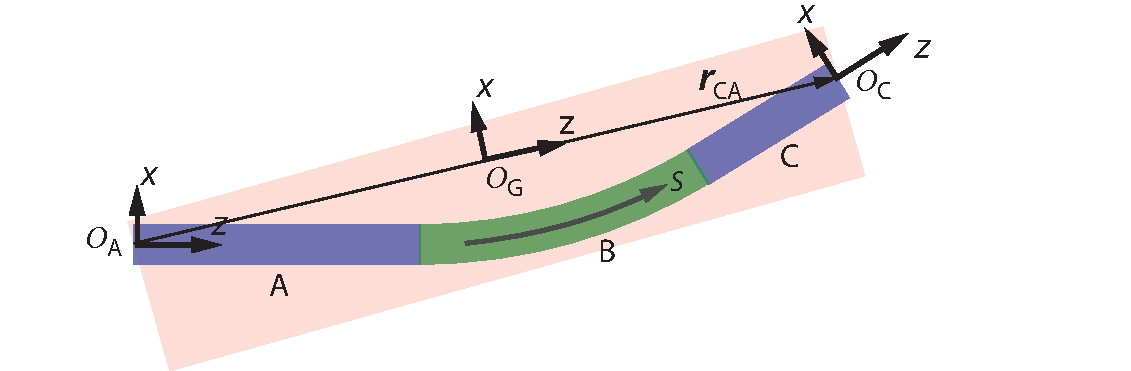
\includegraphics{girder.pdf}
  \caption[Girder example.] {
Girder supporting three elements labeled \vn{A}, \vn{B}, and \vn{C}.
$\calO_A$ is the reference frame at the upstream end of element
\vn{A}, $\calO_C$ is the reference frame at the downstream end of
element \vn{C}, and $\calO_G$ is the default \vn{origin} reference frame of
the girder. $r_{CA}$ is the vector from $\calO_A$ to $\calO_C$.
  }
  \label{f:girder}
\end{figure}

A \vn{girder} is a support structure that orients the elements that
are attached to it in space. A girder can be used to simulate any
rigid support structure and there are no restrictions on how the lattice
elements that are supported are oriented with respect to one another.
Thus, for example, optical tables can be simulated.

General \vn{girder} attributes are:
\begin{center}
\tt
\begin{tabular}{|l|l||l|l|} \hline
  {\sl Attribute Class}  & \s              & {\sl Attribute Class}      & \s              \HH
  Description strings    & \ref{s:alias}   & Offsets, pitches, \& tilt  & \ref{s:offset}  \HH 
\end{tabular}
\end{center}
\toffset

Attributes specific to a \vn{girder} are:
\index{origin_ele}\index{origin_ele_ref_pt}
\index{x_origin}\index{y_origin}
\index{z_origin}\index{theta_origin}
\index{phi_origin}\index{psi_origin}
Attributes specific to a \vn{floor_shift} elements are:
\begin{example}
  girder = \{<List>\}   ! List of elements on the Girder
  origin_ele        = <Name>     ! Reference element.
  origin_ele_ref_pt = <location> ! Reference pt on reference ele.
  dx_origin         = <Real>     ! x-position offset
  dy_origin         = <Real>     ! y-position offset
  dz_origin         = <Real>     ! z-position offset
  dtheta_origin     = <Real>     ! orientation angle offset.
  dphi_origin       = <Real>     ! orientation angle offset.
  dpsi_origin       = <Real>     ! orientation angle offset.
  ds_girder         = <Real>     ! ``Path length'' of girder. Dependent attrib (\sref{s:depend}).
\end{example}

A simple example of a girder is shown in \fig{f:girder}. Here a girder
supports three elements labeled \vn{A}, \vn{B}, and \vn{C} where
\vn{B} is a bend so the geometry is nonlinear. Such a girder may
specified in the lattice file like:
\begin{example}
  g1: girder = \{A, B, C\}
\end{example}
A lattice element may have at most one \vn{girder} supporting it. However, 
a \vn{girder} can be supported by another \vn{girder} which in turn can
be supported by a third \vn{girder}, etc.

The \vn{girder} statement syntax is:
\begin{example}
  <element_name>: GIRDER = \{<ele1>, <ele2>, ..., <eleN> \}, ...
\end{example}
A \vn{girder} element will be created for each section of the lattice
where there is a ``consecutive'' sequence of ``slave'' elements
\vn{<ele1>} through \vn{<eleN>}.  This section of the lattice from
\vn{<ele1>} through \vn{<eleN>} is called the ``girder support
region''.  ``Consecutive'' here means there are no other elements in the
girder support region except for possibly \vn{drift} and/or \vn{marker}
elements.  \vn{Drift} elements cannot be controlled by a girder but may
appear in the girder slave list. If a drift-like element is
desired, use a \vn{pipe} element instead. \vn{Marker} elements present
in a girder support region, but not mentioned in the girder slave
list, are simply ignored.

Wild card characters (\sref{s:lat.attribs}) can be used in any element
name in the girder slave list. Additionally, beam line names
(\sref{s:lines.wo.arg}) can be used. In this case, any \vn{drift} elements
within a beam line will be ignored.

The reference frame from which the girder's offset, pitch, and tilt
attributes (\sref{s:offset}) are measured is constructed as follows: A
reference frame, called the ``\vn{origin}'' reference frame may be
defined using the attributes \vn{origin_ele} and
\vn{origin_ele_ref_pt} which constructs the girder's
\vn{origin} frame to be coincident with the reference frame of another
element. Example:
\begin{example}
  g2: girder = \{...\}, origin_ele = Q, origin_ele_ref_pt = entrance_end
\end{example}
In this example, girder \vn{g2} has an \vn{origin} reference frame
coincident with the entrance end frame of an element named
\vn{Q}. Valid \vn{origin_ele_ref_pt} values are
\begin{example}
  entrance_end
  center        ! Default
  exit_end
\end{example}

If \vn{origin_ele} is not given, the default \vn{origin} frame is
used. The default \vn{origin} frame is constructed as follows:
Let $\calO_A$ be the reference frame of the upstream end of
the first element in the list of supported elements. In this example
it is the upstream end of element \vn{A} as shown in the figure. Let
$\calO_C$ be the downstream end of the last element in the list of
supported elements. In this example this is the downstream end of
element \vn{C}. The origin of the \vn{girder}'s reference frame,
marked $\calO_G$ in the figure, will be half way along the vector
$r_{CA}$ from the origin of $\calO_A$ to the origin of $\calO_B$.  The
orientation of $\calO_G$ is constructed by rotating the $\calO_A$
coordinate system along an axis in $\calO_A$'s $x$-$y$ plane such that
$\calO_A$'s $z$ axis ends up parallel with $r_{CA}$. In the example
above, the rotation axis will be along $\calO_A$'s $y$-axis.

Once the \vn{origin} reference frame is established, the reference
frame of the girder can be offset
from the \vn{origin} frame using the parameters
\begin{example}
  dx_origin    dtheta_origin
  dy_origin    dphi_origin
  dz_origin    dpsi_origin
\end{example} 
The orientation of the \vn{girder}'s reference frame from the \vn{origin}
frame is given in \sref{s:patch.coords}. Example:
\begin{example}
  g3: girder = \{ ... \}, dx_origin = 0.03
\end{example}
This offsets girder \vn{g3}'s reference frame 3~cm horizontally from
the default \vn{origin} frame. If no offsets are given, the
\vn{origin} frame is the same as the girder's reference frame.

\index{x_offset}\index{y_offset}\index{x_pitch}\index{y_pitch}\index{tilt}
The physical orientation of the girder with respect to it's reference
frame is, like other elements, determined by the offset, pitch and
tilt orientation attributes as outlined in \sref{s:offset} and
\sref{s:patch.coords}.  When a girder is shifted in space, the elements
it supports are also shifted.  In this case, the orientation
attributes (\vn{x_offset}, \vn{y_pitch}, etc.) give the orientation of
the element with respect to the \vn{girder}. The orientation with
respect to the local reference coordinates is given by
\vn{x_offset_tot}, which are computed from the orientation attributes
of the element and the \vn{girder}. An example will make this clear:
\begin{example}
  q1: quad, l = 2
  q2: quad, l = 4, x_offset = 0.02, x_pitch = 0.01
  d: drift, l = 8
  g4: girder = \{q1, q2\}, x_pitch = 0.002, x_offset = 0.03
  this_line: line = (q1, d, q2)
  use, this_line
\end{example}
\index{overlay}
In this example, \vn{g4} supports quadrupoles \vn{q1} and \vn{q2}.
Since the supported elements are colinear, the computation is greatly
simplified. The reference frame of \vn{g4}, which is the default
\vn{origin} frame, is at $s = 7$~meters which is half way between the
start of \vn{q1} at at $s = 0$~meters and the end of \vn{q2}) which is
at $s = 14$. The reference frames of \vn{q1} and \vn{q2} are at their
centers so the $s$ positions of the reference frames is
\begin{example}
  Element        S_ref   dS_from_g4
  q1             1.0     -6.0
  g4             7.0      0.0
  q2            12.0      5.0
\end{example}
Using a small angle approximation to simplify the calculation, the
\vn{x_pitch} of \vn{g4} produces an offset at the center of \vn{q2} of
$0.01 = 0.002 * 5$. This, added to the offsets of \vn{g4} and \vn{q2},
give the total offset of \vn{q2} to be $0.06 = 0.01 + 0.03 + 0.02$.
The total \vn{x_pitch} of \vn{q2} is $0.022 = 0.02 + 0.001$.

%-----------------------------------------------------------------------------
\section{Group}
\label{s:group}
\index{group|hyperbf}

\vn{Group} elements are a type of \vn{control} element
(\sref{s:lord.slave}) used to make variations in the attributes of
other elements during execution of a program. For example, to simulate
the action of a control room knob that changes the beam tune in a
storage ring, a \vn{Group} can be used to vary the strength of
selected quads in a specified manner. Also see \vn{overlay}
(\sref{s:overlay}) The difference between \vn{group} and \vn{overlay}
elements is that \vn{overlay} elements set the values of the
attributes directly while \vn{group} elements make changes to
attribute values.

General \vn{girder} attributes are:
\begin{center}
\tt
\begin{tabular}{|l|l||l|l|} \hline
  {\sl Attribute Class}  & \s              & {\sl Attribute Class}      & \s              \HH
  Description strings    & \ref{s:alias}   &                            &                 \HH 
\end{tabular}
\end{center}
\toffset

\index{old_command}\index{command}
\index{coef}\index{type}
\index{alias}\index{descrip}
Attributes specific to a \vn{Group} element are:
\begin{example}
  command     = <Real>    ! Command value.
  old_command = <Real>    ! Old command value.
  coef        = <Real>    ! Conversion factor. Not used by Bmad.  
\end{example}
The \vn{coef} attribute is not used by any \bmad routine. It is
defined for individual programs to store, say, a needed conversion
factor.

The general syntax for a \vn{group} element is
\begin{example}
  name: GROUP = \{ele1[attrib1]:coef1, ele2[attrib2]:coef2, ...\}, 
                                                  default_attrib = init_value
\end{example}
\vn{name} is the name of the \vn{group}, the list in brackets \{...\}
is a list of element attributes to vary along with the coefficients
used for the variation. In any item \vn{ele[attrib]:coef} in the list,
both \vn{attrib} and \vn{coef} are optional. If not present,
\vn{attrib} will default to \vn{default_attrib}. If not present,
\vn{coef} will default to 1. Finally, \vn{init_value} is the initial
value to use for the \vn{group}.

A \vn{group} element is like an \vn{overlay} element in that a
\vn{group} element controls the attribute values of other ``slave''
elements. A \vn{group} element is used to make changes in value. This
is unlike an \vn{overlay} which sets a specific value directly. An
example will make this clear
\begin{example}
  gr: group = \{q1\}, k1 
  gr[command] = 0.34 
  q1, quad, l = ...
  q1[k1] = 0.57
\end{example}
In this example the group \vn{gr} controls the \vn{k1} attribute of
the element \vn{q1}. Unlike overlays, values are assigned to group
elements using the \vn{command} attribute. When a lattice file is
read in then command values for any groups are always applied
last. This is independent of the order that they appear in the file.
Thus in this example the value of q1[k1] would be $0.91 = 0.57 + 0.34$.
When the changes are made to the slave attributes the value of
\vn{command} is stored in the \vn{group}'s \vn{old_command} attribute.
After the lattice is read in a program can change the \vn{gr[command]}
attribute and this change will be added to the value of
\vn{q1[k1]}. The bookkeeping routine that transfers the change from
\vn{gr[command]} to \vn{q1[k1]} doesn't care what the current value of
\vn{q1[k1]} is. It only knows it has to change it by the change in
\vn{gr[command]}.

A \vn{group} will control all elements of a given name. Thus, in
the above example, if there are multiple elements named \vn{q1}
then \vn{gr} will control the \vn{k1}  attribute of all of them.

\index{accordion_edge}\index{start_edge}
\index{end_edge}\index{symmetric_edge}
\index{z_offset}
A \vn{group} can be used to control an elements position and length
using the following as the \vn{default_attrib}
\begin{example}
  accordion_edge  ! Element grows or shrinks symmetrically
  start_edge      ! Varies element's upstream edge s-position
  end_edge        ! Varies element's downstream edge s-position
  symmetric_edge  ! Varies element's overall s-position. Constant length.
  z_offset        ! Similar to symmetric_edge
\end{example}
With \vn{accordion_edge}, \vn{start_edge}, \vn{end_edge}, and
\vn{symmetric_edge} the longitudinal position of an elements edges are
varied. This is done by appropriate control of the element's length
and the lengths of the elements to either side. With \vn{z_offset} the
physical element is offset from its reference position
(\sref{s:offset}) and the elements on either side are untouched.
In all cases the total length of the lattice is kept invariant.

As an example, consider \vn{accordion_edge} which varies the edges of
an element so that the center of the element is fixed but the length
varies. With \vn{accordion_edge} a change of, say, 0.1 in a
\vn{group}'s \vn{command} attribute moves both edges of the element by
0.1 meters so that the length of the element changes by 0.2 meters. To
keep the total lattice length invariant the lengths of the elements to
either side are varied accordingly. For example
\begin{example}
  q10: quad, l = ...
  q11: quad, l = ...
  d1: drift, l = ...
  d2: drift, l = ...
  this_line: line = (... d1, q10, d2, q11, ...)
  gr2: group = \{q10\}, start_edge = 0.1
\end{example}
This last line that defines \vn{gr2} is just a shorthand notation for
\begin{example}
  gr2: group = \{q10\}, start_edge 
  gr2[command] = 0.1
\end{example}
The effect will be to lengthen the length of \vn{q10} and shorten the
length of \vn{d1}.

Like \vn{overlay}s, coefficients can be specified for the individual
elements under a \vn{group}'s control and \vn{group}s can control more
than one type of attribute. For example
\begin{example}
  gr3: group = \{q1[k1]:-1.0, q2[tilt], oct1:-2.0\}, k3
  gr3[command] = 2.0
  gr3[old_command] = 1.5
\end{example}
In this example \vn{gr3} controls 3 attributes of 3 different
elements. The change in \vn{gr3} when the lattice is read in is $0.5
= 2.0 - 1.5$. this 0.5 change will change \vn{q1[k1]} by $-0.5 = -1
\times 0.5$, \vn{q2[tilt]} will change by 0.5 and \vn{oct1[k3]} will
change by $-1.0 = -2.0 * 0.5$.

\index{overlay}\index{girder}
Different \vn{group} elements may control the same element
attribute. And a \vn{group} element may control other \vn{group}
\vn{overlay} or \vn{girder} elements. However, It does not make sense
for a \vn{group} element to control the same attribute as an
\vn{overlay} element or for a \vn{group} element to control a
\vn{dependent} attribute (\sref{s:depend}).

%-----------------------------------------------------------------
\section{Hybrid}
\label{s:hybrid}
\index{hybrid|hyperbf}

A \vn{hybrid} element is an element that is formed by concatenating
other element together. \vn{hybrid} elements are not part of the input
lattice file but are created by a program, usually for speed purposes.

%-----------------------------------------------------------------
\section{Init_Ele}
\label{s:init.ele}
\index{init_ele|hyperbf}

An \vn{init_ele} element, named \vn{BEGINNING}, is placed at the
beginning of every branch (\sref{s:branch}) of a lattice to mark
the start of the branch. The \vn{init_ele} always has element index 0
(\sref{c:lat.concepts}).

\vn{init_ele} attributes are generally set using either \vn{parameter}
(\sref{s:param}) or \vn{beginning} (\sref{s:beginning}) statements.
In particular the initial energy may be set (\sref{s:energy}).

%-----------------------------------------------------------------
\section{Instrument, Monitor, and Pipe}
\label{s:monitor}
\index{instrument|hyperbf}
\index{monitor|hyperbf}
\index{pipe|hyperbf}

Essentially \bmad treats \vn{instrument}, \vn{monitor}, and \vn{pipe}
elements like a \vn{drift}. There is a difference, however, when
superimposing elements (\sref{s:super}). For example, a
\vn{quadrupole} superimposed on top of a \vn{drift} results in a free
\vn{quadrupole} element in the tracking part of the lattice and no
lord elements are created. On the other hand, a \vn{quadrupole}
superimposed on top of a \vn{monitor} results in a \vn{quadrupole}
element in the tracking part of the lattice and this \vn{quadrupole}
element will have two lords: A \vn{quadrupole} superposition lord and
a \vn{monitor} superposition lord.

General \vn{instrument}, \vn{monitor}, and \vn{pipe} attributes are:
\begin{center}
\tt
\begin{tabular}{|l|l||l|l|} \hline
  {\sl Attribute Class}  & \s                  & {\sl Attribute Class}      & \s              \HH
  Symplectify            & \ref{s:symp}        & Offsets, pitches, \& tilt  & \ref{s:offset}  \HH
  Reference energy       & \ref{s:energy}      & Tracking \& transfer map   & \ref{c:methods} \HH
  Aperture Limits        & \ref{s:limit}       & Length                     & \ref{s:l}       \HH
  Description strings    & \ref{s:alias}      & Is_on                      & \ref{s:is.on}   \HH 
  Integration settings   & \ref{s:integ}       & Hkick \& Vkick             & \ref{s:kick}    \HH
  Instrumental variables & \ref{s:meas.attrib} & Chamber wall               & \ref{s:wall}    \HH
\end{tabular}
\end{center}
\toffset

\index{x_offset}
\index{y_offset}
\index{x_pitch}
\index{y_pitch}
\index{tilt}
The \vn{offset}, \vn{pitch}, and \vn{tilt} attributes are not
used by any \bmad routines. If these attributes are used by a program
they are typically used to simulate such things as measurement
offsets. The \vn{is_on} attribute is also not used by \bmad
proper. Example:
\begin{example}
  d21: instrum, l = 4.5
\end{example}

%-----------------------------------------------------------------
\section{Kickers: Hkicker and Vkicker}
\label{s:hvkicker}
\index{hkicker|hyperbf}
\index{vkicker|hyperbf}

An \vn{hkicker} gives a beam a horizontal kick and a \vn{vkicker} gives a 
beam a vertical kick. Also see the \vn{kicker} (\sref{s:kicker}) element.

General \vn{hkicker} \vn{vkicker} attributes are:
\begin{center}
\tt
\begin{tabular}{|l|l||l|l|} \hline
  {\sl Attribute Class}  & \s              & {\sl Attribute Class}      & \s              \HH
  a$n$, b$n$ multipoles      & \ref{s:multip}    & Integration settings       & \ref{s:integ}   \HH
  Aperture Limits            & \ref{s:limit}     & Is_on                      & \ref{s:is.on}   \HH
  Chamber wall               & \ref{s:wall}      & Length                     & \ref{s:l}       \HH
  Description strings        & \ref{s:alias}     & Offsets, pitches, \& tilt  & \ref{s:offset}  \HH
  Field table or map         & \ref{s:em.fields} & Reference energy           & \ref{s:energy}  \HH 
  Fringe Fields              & \ref{s:fringe}    & Symplectify                & \ref{s:symp}    \HH
  Hkick \& Vkick             & \ref{s:kick}      & Tracking \& transfer map   & \ref{c:methods} \HH
\end{tabular}
\end{center}
\toffset

\index{kick}
\index{hkick}
\index{vkick}
Note that \vn{hkicker} and \vn{vkicker} elements use the
\vn{kick} attribute while a \vn{kicker} uses the \vn{hkick} and \vn{vkick} 
attributes. Example:
\begin{example}
  h_kick: hkicker, l = 4.5, kick = 0.003
\end{example}

%-----------------------------------------------------------------
\section{Kicker}
\label{s:kicker}
\index{kicker|hyperbf}

\index{hkick}\index{vkick}
\index{h_displace}\index{v_displace}
A \vn{kicker} can deflect a beam in both planes. Note that a
\vn{kicker} uses the \vn{hkick} and \vn{vkick} attributes while
\vn{hkicker} and \vn{vkicker} elements use the \vn{kick} attribute. 
In addition, a \vn{kicker} can apply a displacement to a particle
using the \vn{h_displace} and \vn{v_displace} attributes.

General \vn{kicker} attributes are:
\begin{center}
\tt
\begin{tabular}{|l|l||l|l|} \hline
  {\sl Attribute Class}      & \s              & {\sl Attribute Class}        & \s              \HH
  a$n$, b$n$ multipoles      & \ref{s:multip}    & Integration settings       & \ref{s:integ}   \HH
  Aperture Limits            & \ref{s:limit}     & Is_on                      & \ref{s:is.on}   \HH
  Chamber wall               & \ref{s:wall}      & Length                     & \ref{s:l}       \HH
  Description strings        & \ref{s:alias}     & Offsets, pitches, \& tilt  & \ref{s:offset}  \HH
  Field table or map         & \ref{s:em.fields} & Reference energy           & \ref{s:energy}  \HH 
  Fringe Fields              & \ref{s:fringe}    & Symplectify                & \ref{s:symp}    \HH
  Hkick \& Vkick             & \ref{s:kick}      & Tracking \& transfer map   & \ref{c:methods} \HH
\end{tabular}
\end{center}
\toffset

Example:
\begin{example}
  a_kick: kicker, l = 4.5, hkick = 0.003
\end{example}

%-----------------------------------------------------------------
\section{Lcavity}
\label{s:lcav}
\index{lcavity|hyperbf}

An \vn{lcavity} is a LINAC accelerating cavity.
The main difference between an \vn{rfcavity} and an
\vn{lcavity} is that, unlike an \vn{rfcavity}, the reference energy
(\sref{s:phase.space}) through an \vn{lcavity} is not constant.

General \vn{lcavity} attributes are:
\begin{center}
\tt
\begin{tabular}{|l|l||l|l|} \hline
  {\sl Attribute Class}      & \s                & {\sl Attribute Class}      & \s                 \HH
  Aperture Limits            & \ref{s:limit}     & Length                     & \ref{s:l}          \HH
  Chamber wall               & \ref{s:wall}      & Offsets, pitches, \& tilt  & \ref{s:offset}     \HH
  Description strings        & \ref{s:alias}     & Reference energy           & \ref{s:energy}     \HH 
  Field table or map         & \ref{s:em.fields} & RF Couplers                & \ref{s:rf.coupler} \HH
  Fringe Fields              & \ref{s:fringe}    & RF Wakes                   & \ref{s:rf.wakes}   \HH
  Hkick \& Vkick             & \ref{s:kick}      & Symplectify                & \ref{s:symp}       \HH
  Integration settings       & \ref{s:integ}     & Tracking \& transfer map   & \ref{c:methods}    \HH
  Is_on                      & \ref{s:is.on}     &                            &                    \HH
\end{tabular}
\end{center}
\toffset

The attributes specific to an \vn{lcavity} are 
\index{gradient}\index{phi0}\index{n_cell}
\index{dphi0}\index{e_loss}
\index{rf_frequency}\index{voltage}
\begin{example}
  gradient       = <Real>    ! Accelerating gradient (V/m).
  gradient_err   = <Real>    ! Accelerating gradient error (V/m).
  phi0           = <Real>    ! Phase (rad/2\(\pi\)) of the reference particle with 
                             !   respect to the RF. phi0 = 0 is on crest.
  dphi0          = <Real>    ! Phase with respect to a multipass lord (rad/2\(\pi\)).
  phi0_err       = <Real>    ! Phase error (rad/2\(\pi\))
  dphi0_ref      = <Real>    ! Phase offset used to deal with absolute time tracking
                             !  and other issues (see below).
  e_loss         = <Real>    ! Loss parameter for short range wake fields (V/Coul).
  rf_frequency   = <Real>    ! Rf frequency (Hz).
  voltage                    ! Cavity voltage. Dependent attribute (\sref{s:depend}).
  n_cell         = <Integer> ! Number of cavity cells. Default is 1.
\end{example}
The dependent variable \vn{voltage} attribute can be used in place of
\vn{gradient} as discussed in \sref{s:depend}.  \vn{voltage} is a
dependent attribute and is defined to be
\begin{example}
  voltage = gradient * L
\end{example}

The energy kick felt by a particle, assuming no phase slippage, is 
\begin{example}
  dE = gradient_tot * L * cos(twopi * (phi_particle + phi_ref))
\end{example}
\index{multipass}
where the total gradient is
\begin{example}
  gradient_tot = gradient + gradient_err
\end{example}
the phase \vn{phi_ref} is
\begin{example}
  phi_ref = phi0 + dphi0 + phi0_err + dphi0_ref
\end{example}
and \vn{phi_particle} is
\begin{example}
  phi_particle = -z * rf_frequency / velocity  ! With relative time tracking (\sref{s:rf.time})
               =  t_particle * rf_frequency    ! With absolute time tracking
\end{example}
With \vn{relative time tracking}, the phase, \vn{phi_particle}, of the
particle with respect to the cavity's internal clock is proportional
to \vn{z} -- the particles' phase space coordinate
(\sref{s:phase.space}). With \vn{absolute time tracking},
\vn{phi_particle} is proportional to the absolute time the particle
reaches the cavity. See section~\sref{s:rf.time} for a discussion on
relative verses absolute time tracking. The switch to set the type of
tracking for a lattice is \vn{parameter[absolute_time_tracking]}
(\sref{s:param}).

\vn{dphi0} is only to be used to shift the phase with respect to a
\vn{multipass} lord. See \sref{s:multipass}.

\vn{dphi0_ref} is a phase calculated by \bmad's RF auto-phase module
(\sref{s:em.fields}).

The energy change of the reference particle is just the energy change for a 
particle with $z = 0$ and no phase or gradient errors. Thus
\begin{example}
  dE(reference) = gradient * L * cos(twopi * phi_ref)
\end{example}

The energy kick for a \bmad \vn{lcavity} is consistent with MAD. 
Note: The MAD8 documentation for an \vn{lcavity} has a wrong
sign. Essentially the MAD8 documentation gives
\begin{example}
  dE = gradient * L * cos(twopi * (phi_ref - phi(z))) ! WRONG
\end{example}
This is incorrect. 

When short-range wake fields are being simulated, with
\vn{bmad_com%sr_wakes_on = True} (\sref{s:bmad.params}), the
\vn{e_loss} attribute can be used to modify the gradient in order to
maintain a constant average energy gain. That is, \vn{e_loss} can be
used to simulate the effect of a feedback circuit that attempts to
maintain the average energy of the bunch after the element constant.
The energy kick is then
\begin{example}
  dE(with wake) = dE + e_loss * n_part * e_charge 
\end{example}
\vn{n_part} is set using the \vn{parameter} statement (\sref{s:param})
and represents the number of particles in a bunch. \vn{e_charge} is
the charge on an electron (Table~\ref{t:constants}). Notice that the
\vn{e_loss} term is independent of the sign of the charge of the particle.

The transverse trajectory through an \vn{lcavity} is modeled using
equations developed by Rosenzweig and Serafini\cite{b:rosenzweig}
modified to give the correct phase-space area at non
ultra-relativistic energies.  See Section \sref{s:lcav.phys} for more
details.  Note: The transfer matrix for an \vn{lcavity} with finite
\vn{gradient} is never symplectic. See \sref{s:phase.space}. In
addition, couplers (\sref{s:rf.coupler}) and HOM wakes
(\sref{s:rf.wakes}) can be modeled.

When using \vn{boris} or \vn{runge_kutta}, tracking (\sref{s:tkm})
through a field map (\sref{s:em.fields}), the \vn{bmad_standard} field
is \vn{n_cell} half wave resonators.

Example:
\begin{example}
  lwf: lcavity, l = 2.3, rf_frequency = 500e6, voltage = 20e6
\end{example}

%-----------------------------------------------------------------
\section{Marker}
\label{s:mark}
\index{marker|hyperbf}

A \vn{marker} is a zero length element meant to mark a position. 

General \vn{marker} attributes are:
\begin{center} 
\tt
\begin{tabular}{|l|l||l|l|} \hline
  {\sl Attribute Class}  & \s                  & {\sl Attribute Class}      & \s              \HH
  Description strings    & \ref{s:alias}      & Is_on                      & \ref{s:is.on}   \HH 
  Reference energy       & \ref{s:energy}      & Offsets \& tilt            & \ref{s:offset}  \HH
  Aperture Limits        & \ref{s:limit}       & Tracking \& transfer map   & \ref{c:methods} \HH
  Instrumental variables & \ref{s:meas.attrib} &                            &                 \HH
\end{tabular}
\end{center}
\toffset

\index{x_ray_line_len}
Attributes specific to a \vn{marker} element are:
\begin{example}
  x_ray_line_len = <Real>
\end{example}
\vn{x_ray_line_len} is the length of an associated x-ray synchrotron
light line measured from the marker element. This is used for
machine geometry calculations and is irrelevant for lattice
computations.

\index{x_offset}\index{y_offset}
\index{tilt}\index{is_on}
The \vn{x_offset}, \vn{y_offset} and \vn{tilt} attributes are not used
by any \bmad routines. Typically, if these attributes are used by a
program, they are used to simulate things like BPM offsets. The
\vn{is_on} attribute is also not used by \bmad proper. 

Example:
\begin{example}
  mm: mark, type = "BPM"
\end{example}

%-----------------------------------------------------------------
\section{Match}
\label{s:match}
\index{match|hyperbf}

A \vn{match} element is used to match the Twiss parameters between two
points. 

General \vn{match} attributes are:
\begin{center} 
\tt
\begin{tabular}{|l|l||l|l|} \hline
  {\sl Attribute Class}  & \s              & {\sl Attribute Class}      & \s              \HH
  Description strings    & \ref{s:alias}  & Is_on                      & \ref{s:is.on}   \HH 
  Aperture Limits        & \ref{s:limit}   & Length                     & \ref{s:l}       \HH
  Reference energy       & \ref{s:energy}  & Integration settings       & \ref{s:integ}   \HH
\end{tabular}
\end{center}
\toffset

Attributes specific to a \vn{match} element are:
\begin{example}
  beta_a0   = <Real>,  beta_b0  = <Real>   ! Beginning betas
  beta_a1   = <Real>,  beta_b1  = <Real>   ! Ending betas
  alpha_a0  = <Real>,  alpha_b0 = <Real>   ! Beginning alphas
  alpha_a1  = <Real>,  alpha_b1 = <Real>   ! Ending alphas
  eta_x0    = <Real>,  eta_y0   = <Real>   ! Beginning etas 
  eta_x1    = <Real>,  eta_y1   = <Real>   ! Ending etas 
  etap_x0   = <Real>,  etap_y0  = <Real>   ! Beginning eta' 
  etap_x1   = <Real>,  etap_y1  = <Real>   ! Ending eta'
  dphi_a    = <Real>,  dphi_b   = <Real>   ! Phase advances
  match_end = <Logic>                      ! See below. Default is False.
  x0, px0, y0, py0, z0, pz0 = <Real>       ! Beginning coordinates
  x1, px1, y1, py1, z1, pz1 = <Real>       ! Ending coordinates
  match_end_orbit = <Logic>                ! See below. Default is False.
\end{example}

\index{beta_a0}\index{beta_b0}
\index{beta_a1}\index{beta_b1}
\index{eta_x0}\index{etap_x0}
\index{eta_y0}\index{etap_y0}
\index{dphi_a}\index{dphi_b}
The transfer map for a \vn{match} element, which is just a
linear matrix, is calculated such that if the Twiss parameters at the
exit end of the element preceding the \vn{match} element are given by
\vn{beta_a0}, \vn{beta_b0}, etc., then the computed Twiss parameters
at the exit end of the \vn{match} element will be \vn{beta_a1},
\vn{beta_b1}, etc., and the phase advances (in radians) will be \vn{dphi_a} and \vn{dphi_b}.

\index{x0}\index{px0}\index{y0}\index{py0}\index{z0}\index{pz0}
\index{x1}\index{px1}\index{y1}\index{py1}\index{z1}\index{pz1}
The coordinate parameters (\vn{x0}, \vn{x1}, etc.) add a constant term
(a ``kick'') to the transfer map through a \vn{match} element:
\Begineq
  r_1 = \Bf M \, r_0 + \Bf V 
\Endeq
where $r_1$ is the output coordinates, $r_0$ are the input
coordinates, $\Bf M$ is the transfer matrix determined by the settings
of the beginning and ending twiss and dispersion attributes, and the
kick term, $\Bf V$ is given by
\Begineq
  \Bf V = 
    \begin{pmatrix} 
    \mbox{x1} \\ \mbox{px1} \\ \mbox{y1} \\ \mbox{py1} \\ \mbox{z1} \\ \mbox{pz1} 
    \end{pmatrix} -
    \Bf M \, \begin{pmatrix} 
    \mbox{x0} \\ \mbox{px0} \\ \mbox{y0} \\ \mbox{py0} \\ \mbox{z0} \\ \mbox{pz0} 
    \end{pmatrix}
\Endeq

\index{l}
The attribute \vn{l} is not used in the transfer matrix
calculation. It is sometimes needed by a program for other
computations. For example, to compute the time it takes to go through
a match element.

Example:
\begin{example}
  mm: match, beta_a0 = 12.5, beta_b0 = 3.4, eta_x0 = 1.0, ...
\end{example}

  \begin{description} 
  \index{open}
  \index{match_end}
  \item[Match_end] \Newline
The \vn{match_end} attribute is used for setting the beginning Twiss
attributes (\vn{beta_a0}, \vn{alpha_a0}, etc.) from within a
program. If the \vn{match_end} attribute is set to True, the beginning
Twiss attributes are set to be equal to the Twiss parameters from the
exit end of the previous element. That is, when the Twiss parameters
are calculated, the calculated Twiss parameters at the exit end of the
match element will be the exit Twiss attributes (\vn{beta_a1},
\vn{alpha_a1}, etc.) as set in the \vn{match} element. The
\vn{match_end} attribute may only be used with \vn{open}
lattices (\sref{s:param}) since, for a \vn{closed}, it is
not possible to calculate the Twiss parameters at the previous element
independently of the exit Twiss attributes at the \vn{match} element.

When running a program, if a \vn{match} element initially has it's
\vn{match_end} attribute is set to True, the \bmad bookkeeping
routines will ensure that the \vn{match} element's beginning Twiss
attributes are appropriately set as explained above. If \vn{match_end}
is now toggled to False, the beginning Twiss attribute values, and
hence the transfer matrix for the \vn{match} element, will be
frozen. Variation now of any parameter in the lattice that
affects the calculated Twiss parameters through the \vn{match}
element will not affect the \vn{match} element's transfer matrix.

  \index{match_end_orbit}
  \item[match_end_orbit]
The \vn{match_end_orbit} attribute is similar to the \vn{match_end}
attribute.  When running a program, if \vn{match_end_orbit} is set to
True, when any particle is tracked through the \vn{match} element, the
\vn{match} element's starting coordinate attributes, \vn{(x0, px0, y0,
py0, z0, pz0)}, will be set to the particle's coordinates at the exit
end of the previous element. That is, the particle will always have
coordinates equal to \vn{(x1, px1, y1, py1, z1, pz1)} at the end of
the \vn{match} element.  If \vn{match_end_orbit} is now toggled to
False, the ending coordinate attributes, and hence the $\Bf V$ vector,
will become fixed. As with the \vn{match_end} attribute, the
\vn{match_end_orbit} attribute may only be used with \vn{open}
lattices (\sref{s:param}).


\end{description}

%-----------------------------------------------------------------
\section{Mirror}
\label{s:mirror}
\index{mirror|hyperbf}

A \vn{mirror} reflects photons. 

General \vn{mirror} attributes are:
\begin{center}
\tt 
\begin{tabular}{|l|l||l|l|} \hline
  {\sl Attribute Class}  & \s              & {\sl Attribute Class}      & \s              \HH
  Description strings    & \ref{s:alias}  & Offsets, pitches, \& tilt  & \ref{s:offset}  \HH
  Reference energy       & \ref{s:energy}  & Tracking \& transfer map   & \ref{c:methods} \HH
  Aperture Limits        & \ref{s:limit}   & Chamber wall               & \ref{s:wall}    \HH
  Surface Curvature      & \ref{s:s.curve} &                            &                 \HH
\end{tabular}
\end{center}
\toffset

Attributes specific to a \vn{mirror} element are:
\begin{example}
  graze_angle     = <Real>    ! Angle between incoming beam and mirror surface.
  critical_angle  = <Real>    ! Critical angle.
  tilt_err        = <Real>    ! Error in the tilt angle.
\end{example}

The reference trajectory for a
\vn{mirror} is that of a zero length bend (\sref{s:mirror.coords}) and
hence the length (\vn{l}) parameter of a mirror is fixed at zero. The
reference trajectory is determined by the values of the
\vn{graze_angle} and \vn{tilt} parameters. A positive \vn{graze_angle}
bends the reference trajectory in the same direction as a positive
\vn{g} for a bend element.

A \vn{mirror} may be offset and pitched (\ref{s:offset}). The incoming
local reference coordinates are used for these misalignments.

%-----------------------------------------------------------------
\section{Multipole}
\label{s:mult}
\index{multipole|hyperbf}

A \vn{multipole} is a thin multipole lens up to 20th order. The basic
difference between this and an \vn{ab_multipole} is the input
format. See section~\sref{s:fields} for how the multipole coefficients
are defined.

General \vn{multipole} attributes are:
\begin{center}
\tt 
\begin{tabular}{|l|l||l|l|} \hline
  {\sl Attribute Class}  & \s              & {\sl Attribute Class}      & \s              \HH
  K$n$L, T$n$ multipoles & \ref{s:multip}  & Offsets, pitches, \& tilt  & \ref{s:offset}  \HH
  Description strings    & \ref{s:alias}  & Is_on                      & \ref{s:is.on}   \HH 
  Reference energy       & \ref{s:energy}  & Tracking \& transfer map   & \ref{c:methods} \HH
  Aperture Limits        & \ref{s:limit}   &                            &                 \HH
\end{tabular}
\end{center}
\toffset

\index{l}
The length \vn{l} is a fictitious length that is used for synchrotron
radiation computations and affects the longitudinal position of the
next element but does not affect any tracking or transfer map
calculations.

Like a \mad \vn{multipole}, a \bmad \vn{multipole} will affect the
reference orbit if there is a dipole component. 
Example:
\begin{example}
  m1: multipole, k1l = 0.034e-2, t1, k3l = 4.5, t3 = 0.31*pi
\end{example}

%-----------------------------------------------------------------
\section{Multilayer_mirror}
\label{s:multilayer}
\index{multilayer_mirror|hyperbf}

A \vn{multilayer_mirror} is a substrate upon which multiple layers
of alternating substances have been deposited. The idea is similar to crystal
diffraction: light reflected at each interface constructively interferes 
with light reflected from other interfaces. The amplified reflection offsets 
losses due to absorption. 

General \vn{crystal} attributes are:
\begin{center}
\tt
\begin{tabular}{|l|l||l|l|} \hline
  {\sl Attribute Class}  & \s              & {\sl Attribute Class}      & \s              \HH
  Description strings    & \ref{s:alias}  & Offsets                    & \ref{s:offset}  \HH
  Reference energy       & \ref{s:energy}  & Tracking \& transfer map   & \ref{c:methods} \HH
  Aperture Limits        & \ref{s:limit}   & Symplectify                & \ref{s:symp}    \HH
  Chamber Wall           & \ref{s:wall}    & Surface Curvature          & \ref{s:s.curve} \HH
\end{tabular}
\end{center}
\toffset

\index{crystal_type}\index{d1_thickness}\index{d2_thickness}
\index{n_cell}\index{tilt_err}
\index{c2_curve}\index{c3_curve}
\index{c4_curve}\index{d_detec}
\index{d_source}\index{g_trans}
\index{tilt_err}
The attributes specific to a \vn{multilayer_mirror} are 
\begin{example}
  crystal_type         = <String>  ! Materials in each layer.
  d1_thickness         = <Real>    ! Thickness of layer 1
  d2_thickness         = <Real>    ! Thickness of layer 2
  n_cell               = <Integer> ! Number of cells (= Number of layers / 2)
  tilt_err             = <Real>    ! Error in the tilt angle.
\end{example}

\index{graze_angle}\index{c2_curve_tot}
\index{c3_curve_tot}\index{c4_curve_tot}
\index{f0_re1}\index{f0_im1}
\index{f0_re2}\index{f0_im2}
\index{v1_unitcell}\index{v2_unitcell}
Dependent attributes (\sref{s:depend}) are
\begin{example}
  graze_angle      ! Angle between incoming beam and mirror surface.
  f0_re1           ! Real part of f0 for layer 1
  f0_im1           ! Imaginary part of f0 for layer 1
  f0_re2           ! Real part of f0 for layer 2
  f0_im2           ! Imaginary part of f0 for layer 2
  v1_unitcell      ! Unit cell volume for layer 1
  v2_unitcell      ! Unit cell volume for layer 2 
\end{example}

A \vn{multilayer_mirror} is constructed of a number of ``cells''. The
number of cells is set by \vn{n_cell}. Each cell consists of two
layers of dielectric material. The materials used is given by
the \vn{crystal_type} attribute. The format for this is
\begin{example}
  crystal_type = "<material_1>:<material_2>"
\end{example}
where \vn{<material_1>} and \vn{<material_2>} are the material names
for the first and second layers of the cell respectively. The first
layer is the bottom layer and the second layer is the top layer of the cell.
Material names are case sensitive. So ``FE'' cannot be used in place of ``Fe''

Example:
\begin{example}
  mm: multilayer_mirror, crystal_type = 'W:B4C', n_cell = 100, &
            d1_thickness = 1e-9, d2_thickness = 1.5e-9
\end{example}

%-----------------------------------------------------------------
\section{Null_Ele}
\label{s:null.ele}
\index{null_ele|hyperbf}

A \vn{null_ele} is a special type of element. It is like a \vn{marker}
but it has the property that when the lattice is expanded
(\sref{s:lines.wo.arg}) all \vn{null_ele} elements are removed. The
primary use of a \vn{null_ele} is in computer generated lattices where
it can be used to serve as a reference point for element
superpositions (\sref{s:super}). It is not generally useful otherwise.

%-----------------------------------------------------------------
\section{Octupole}
\label{s:oct}
\index{octupole|hyperbf}

An \vn{octupole} is a magnetic element with a cubic field dependence
with transverse offset (\sref{s:fields}).  The \vn{bmad_standard}
calculation treats an octupole using a kick--drift--kick model.

General \vn{octupole} attributes are:
\begin{center}
\tt
\begin{tabular}{|l|l||l|l|} \hline
  {\sl Attribute Class}      & \s                & {\sl Attribute Class}      & \s              \HH
  a$n$, b$n$ multipoles      & \ref{s:multip}    & Integration settings       & \ref{s:integ}   \HH
  Aperture Limits            & \ref{s:limit}     & Is_on                      & \ref{s:is.on}   \HH
  Chamber wall               & \ref{s:wall}      & Length                     & \ref{s:l}       \HH
  Description strings        & \ref{s:alias}     & Offsets, pitches, \& tilt  & \ref{s:offset}  \HH
  Field table or map         & \ref{s:em.fields} & Reference energy           & \ref{s:energy}  \HH 
  Fringe Fields              & \ref{s:fringe}    & Symplectify                & \ref{s:symp}    \HH
  Hkick \& Vkick             & \ref{s:kick}      & Tracking \& transfer map   & \ref{c:methods} \HH
\end{tabular}
\end{center}
\toffset

\index{k3}
\index{b3_gradient}
Attributes specific to an \vn{octupole} element are:
\begin{example}
  k3          = <Real>   ! Octupole strength.
  b3_gradient = <Real>   ! Field strength. (\sref{s:depend}).
\end{example}

\index{tilt}
If the \vn{tilt} attribute is present without a value then a value of 
$\pi/8$ is used.
Example:
\begin{example}
  oct1: octupole, l = 4.5, k3 = 0.003, tilt ! same as tilt = pi/8
\end{example}

%-----------------------------------------------------------------------------
\section{Overlay}
\label{s:overlay}
\index{ovlerlay|hyperbf}

\vn{Overlay} elements are a type of \vn{control} element
(\sref{s:lord.slave}) used to make variations in the attributes of
other elements while a program is running. For example, to simulate
the action of a magnet power supply that controls a string of
magnets. Also see \vn{group} (\sref{s:group}) The difference between
\vn{group} and \vn{overlay} elements is that \vn{overlay} elements set
the values of the attributes directly while \vn{group} elements make
changes to attribute values.

General \vn{girder} attributes are:
\begin{center}
\tt
\begin{tabular}{|l|l||l|l|} \hline
  {\sl Attribute Class}  & \s              & {\sl Attribute Class}      & \s              \HH
  Description strings    & \ref{s:alias}   &                            &                 \HH 
\end{tabular}
\end{center}
\toffset

The general syntax for a \vn{overlay} element is
\begin{example}
  name: OVERLAY = \{ele1[attrib1]:coef1, ele2[attrib2]:coef2, ...\}, 
                                                       default_attrib = init_value
\end{example}
\vn{name} is the name of the \vn{overlay}, the list in brackets \{...\}
is a list of element attributes to vary along with the coefficients
used for the variation. In any item \vn{ele[attrib]:coef} in the list,
both \vn{attrib} and \vn{coef} are optional. If not present,
\vn{attrib} will default to \vn{default_attrib}. If not present,
\vn{coef} will default to 1. Finally, \vn{init_value} is the initial
value to use for the \vn{overlay}.

An \vn{overlay} element is used to control the attributes of other elements. 
For example: 
\begin{example}
  over1: overlay = \{a_ele, b_ele:2.0\}, hkick = 0.003
  over2: overlay = \{b_ele\}, hkick
  over2[hkick] = 0.9
  a_ele: quad, hkick = 0.05, ...
  b_ele: rbend, ...
  this_line: line = ( ... a_ele, ... b_ele, ... )
  use, this_line
\end{example}

In the example the overlay \vn{over1} controls the \vn{hkick}
attribute of the "slave" elements \vn{a_ele} and
\vn{b_ele}. \vn{over2} controls the hkick attribute of just
\vn{b_ele}. \vn{over1} has a \vn{hkick} value of 0.003 and \vn{over2}
has been assigned a value for \vn{hkick} of 0.9.

There are coefficients associated with the control of a slave element. 
The default coefficient is 1.0. To specify a coefficient use a vertical colon ":"
after the element name followed by the coefficient. In the above example 
the coefficient for the control of \vn{b_ele} from \vn{over1} is 2.0 
and for the others the default 1.0 is used. thus 
\begin{example}
  a_ele[hkick] = over1[hkick]
               = 0.003
  b_ele[hkick] = over2[hkick] + 2 * over1[hkick] 
               = 0.906
\end{example}
Note: An older notation allowed a slash "/" to be used in place of the
colon ":" for the separator between the slave name and the
coefficient. While the slash is still accepted, its use is
discouraged.

An \vn{overlay} will control all elements of a given name. Thus, in
the above example, if there are multiple elements in the lattice
with the name \vn{b_ele} then the \vn{over1} and \vn{over2} overlays
will control the \vn{hkick} attribute of all of them.

Note: Overlays completely determine the value of the attributes that
are controlled by the overlay. in the above example, the hkick of 0.05
assigned directly to \vn{a_ele} is overwritten by the overlay action
of \vn{over1}.

\noindent The default value for an overlay is 0 so for example
\begin{example}
  over3: overlay = \{c_ele\}, k1
\end{example}
will make \vn{c_ele[k1]} = 0. Overlays can also control more than one
type of attribute as the following example shows
\begin{example}
  over4: overlay = \{this_quad[k1]:5.4, this_sextupole[k2], ...\}, hkick
\end{example}

\index{group}\index{girder}
As illustrated above, different \vn{overlay} elements may control the
same element attribute. And an \vn{overlay} element may control other
\vn{overlay}, \vn{group} or \vn{girder} elements. However, It does not
make sense for an \vn{overlay} element to control the same attribute
as a \vn{group} element or for an \vn{overlay} element to control a
\vn{dependent} attribute (\sref{s:depend}).

%-----------------------------------------------------------------
\section{Patch}
\label{s:patch}
\index{patch|hyperbf}

\begin{figure}[tb]
  \centering
  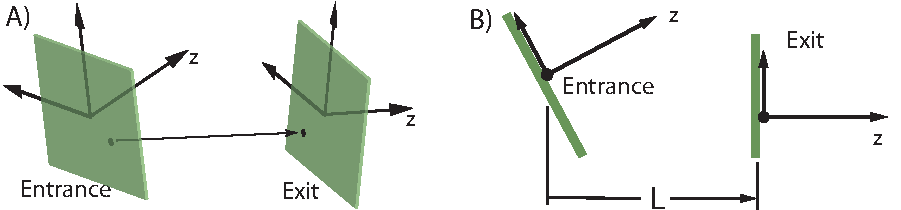
\includegraphics[width=5in]{patch.pdf}
  \caption[Patch transformation.]
{A \vn{patch} element can align its exit face arbitrarily with respect
to its entrance face.}
  \label{f:patch}
\end{figure}

%---------------------------------------------------------------------------------

A \vn{patch} element shifts the reference orbit and time. Also see
\vn{floor_shift} (\sref{s:floor.ele}) and \vn{fiducial}
(\sref{s:fiducial}) elements.

General \vn{patch} element attributes are:
\begin{center}
\tt
\begin{tabular}{|l|l||l|l|} \hline
  {\sl Attribute Class}  & \s              & {\sl Attribute Class}      & \s              \HH
  is_on                  & \ref{s:is.on}   & Offsets, pitches, \& tilt  & \ref{s:offset}  \HH
  Reference energy       & \ref{s:energy}  & Tracking \& transfer map   & \ref{c:methods} \HH
  Aperture Limits        & \ref{s:limit}   & Description strings        & \ref{s:alias}   \HH 
  Length                 & \ref{s:l}       &                            &                 \HH
\end{tabular}
\end{center}
\toffset

\index{flexible}\index\index{e_tot_offset}
\index{x_offset}\index{y_offset}\index{z_offset}\index{tilt}
\index{x_pitch}\index{y_pitch}\index{t_offset}
Attributes specific to a \vn{patch} elements are:
\begin{example}
  x_offset        = <Real>  ! Exit face offset from Entrance.
  y_offset        = <Real>  ! Exit face offset from Entrance.
  z_offset        = <Real>  ! Exit face offset from Entrance.
  t_offset        = <Real>  ! Reference time offset.
  x_pitch         = <Real>  ! Exit face orientation from Entrance.
  y_pitch         = <Real>  ! Exit face orientation from Entrance.
  tilt            = <Real>  ! Exit face orientation from Entrance.
  e_tot_offset    = <Real>  ! Reference energy offset (eV).
  flexible        = <Logic>  ! Default: False.
\end{example}
\index{x_offset}

A straight line element like a \vn{drift} or a \vn{quadrupole} has the
the exit face parallel to the entrance face. With a \vn{patch}
element, the entrance and exit faces can be arbitrarily oriented with
respect to one another as shown in \fig{f:patch}. There are two
different ways the orientation of the exit face is determined. Which
way is determined by the setting of the \vn{flexible} attribute.

\index{rigid patch}\index{infleible patch}
\index{flexible patch}
With the \vn{flexible} attribute set to \vn{False}, the default, The
exit face of the \vn{patch} will be determined from the offset, tilt
and pitch attributes as described in \sref{s:patch.coords}. This type
of \vn{patch} is called ``rigid'' or ``inflexible'' since the geometry
of the \vn{patch} is solely determined by the \vn{patch}'s attributes
and is independent of everything else.
Example:
\begin{example}
  pt: patch, z_offset = 3.2   ! Equivalent to a drift
\end{example}

With \vn{flexible} set to \vn{True}, the exit face is taken to be the
reference frame of the entrance face of the next element in the
lattice. In this case, it must be possible to compute the reference
coordinates of the next element before the reference coordinates of
the \vn{patch} are computed. A \vn{flexible} \vn{patch} will have the
its offsets, pitches, and tilt as dependent parameters
(\sref{s:depend}) and these parameters will be computed. Here the
\vn{patch} is called ``flexible'' since the geometry of the patch will
depend upon the geometry of the rest of the lattice and, therefore, if
the geometry of the rest of the lattice is modified (is ``flexed''),
the geometry of the \vn{patch} will vary as well. See
Section~\sref{s:ex.erl} for an example.

With \vn{bmad_standard} tracking (\sref{s:tkm}) A particle, starting
at the upstream face of the \vn{patch}, is propagated in a straight
line to the downstream face and the suitable coordinate transformation
is made to translate the particle's coordinates from the upstream
coordinate frame to the downstream coordinate frame
(\sref{s:patch.std}). In this case the \vn{patch} element can be
thought of as a generalized \vn{drift} element.

If there are magnetic or electric fields within the \vn{patch}, the
tracking method through the \vn{patch} must be set to either
\vn{runge_kutta} or \vn{custom}. Example:
\begin{example}
  pa2: patch, tracking_method = runge_kutta, field_calc = custom, 
              mat6_calc_method = tracking, ...
\end{example}
In order to supply a custom field when \vn{runge_kutta} tracking is
used, \vn{field_calc} (\sref{s:integ}) needs to be set to
\vn{custom}. In this case, custom code must be supplied for
calculating the fields as a function of position
(\sref{s:custom.ele}).

The \vn{e_tot_offset} attribute offsets the
reference energy:
\begin{example}
  E_tot_ref(exit) = E_tot_ref(entrance) + E_tot_offset (eV)
\end{example}
Setting the \vn{e_tot_offset} attribute will affect a particle's
$p_x$, $p_y$ and $p_z$ coordinates via \Eqs{ppp} and \eq{ppppp}.
Notice that \vn{e_tot_offset} does not affect a particle's actual
energy, it just affects the difference between the particle energy and
the reference energy. 

The \vn{t_offset} attribute offsets the reference time:
\begin{example}
  t_ref(exit) = t_ref(entrance) + t_offset + dt_travel_ref
\end{example}
where \vn{dt_transit_ref} is the time for the reference particle to
travel through the patch.  Setting the \vn{t_offset} attribute will
affect a particle's $z$ coordinate via \Eqs{zbctt}.

When a lattice branch contains both normally oriented and reversed elements
(\sref{s:ref.construct}), a \vn{patch}, (or series of \vn{patches}),
which reflects the $z$ direction must be placed in between. Such a
\vn{patch}, (or patches) is called a \vn{reflection}
\vn{patch}. See Section~\sref{s:reflect.patch} for more details.

%-----------------------------------------------------------------
\section{Quadrupole}
\label{s:quad}
\index{quadrupole|hyperbf}

A \vn{quadrupole} is a magnetic element with a linear field dependence
with transverse offset (\sref{s:fields}).

General \vn{quadrupole} attributes are:
\begin{center}
\tt
\begin{tabular}{|l|l||l|l|} \hline
  {\sl Attribute Class}      & \s                & {\sl Attribute Class}      & \s              \HH
  a$n$, b$n$ multipoles      & \ref{s:multip}    & Integration settings       & \ref{s:integ}   \HH
  Aperture Limits            & \ref{s:limit}     & Is_on                      & \ref{s:is.on}   \HH
  Chamber wall               & \ref{s:wall}      & Length                     & \ref{s:l}       \HH
  Description strings        & \ref{s:alias}     & Offsets, pitches, \& tilt  & \ref{s:offset}  \HH
  Field table or map         & \ref{s:em.fields} & Reference energy           & \ref{s:energy}  \HH 
  Fringe Fields              & \ref{s:fringe}    & Symplectify                & \ref{s:symp}    \HH
  Hkick \& Vkick             & \ref{s:kick}      & Tracking \& transfer map   & \ref{c:methods} \HH
\end{tabular}
\end{center}
\toffset

\index{k1}
\index{b1_gradient}
Attributes specific to a \vn{quadrupole} element are:
\begin{example}
  k1             = <Real>    ! Quadrupole strength.
  b1_gradient    = <Real>    ! Field strength. (\sref{s:depend}).
 \end{example}

\index{tilt}
If the \vn{tilt} attribute is present without a value then a value of $\pi/4$
is used.

For a quadrupole with zero \vn{tilt} and a positive \vn{k1}, the
quadrupole is horizontally focusing and vertically defocusing
(\sref{s:fields}).

Example:
\begin{example}
  q03w: quad, l = 0.6, k1 = 0.003, tilt  ! same as tilt = pi/4
\end{example}

%-----------------------------------------------------------------
\section{RFcavity}
\label{s:rfcav}
\index{rfcavity|hyperbf}

An \vn{rfcavity} is an RF cavity without acceleration generally used
in a storage ring. The main difference between an \vn{rfcavity} and an
\vn{lcavity} is that, unlike an \vn{lcavity}, the reference energy
(\sref{s:phase.space}) through an \vn{rfcavity} is constant.

General \vn{rfcavity} attributes are:
\begin{center}
\tt
\begin{tabular}{|l|l||l|l|} \hline
  {\sl Attribute Class}      & \s                & {\sl Attribute Class}      & \s                 \HH
  Aperture Limits            & \ref{s:limit}     & Length                     & \ref{s:l}          \HH
  Chamber wall               & \ref{s:wall}      & Offsets, pitches, \& tilt  & \ref{s:offset}     \HH
  Description strings        & \ref{s:alias}     & Reference energy           & \ref{s:energy}     \HH 
  Field table or map         & \ref{s:em.fields} & RF Couplers                & \ref{s:rf.coupler} \HH
  Fringe Fields              & \ref{s:fringe}    & RF Wakes                   & \ref{s:rf.wakes}   \HH
  Hkick \& Vkick             & \ref{s:kick}      & Symplectify                & \ref{s:symp}       \HH
  Integration settings       & \ref{s:integ}     & Tracking \& transfer map   & \ref{c:methods}    \HH
  Is_on                      & \ref{s:is.on}     &                            &                    \HH
\end{tabular}
\end{center}
\toffset

\index{rf_frequency}\index{harmon}\index{voltage}\index{phi0}\index{dphi0}
Attributes specific to an \vn{rfcavity} are:
\begin{example}
  rf_frequency = <Real>    ! Frequency
  harmon       = <Real>    ! Harmonic number
  voltage      = <Real>    ! Cavity voltage
  phi0         = <Real>    ! Cavity phase
  dphi0        = <Real>    ! Phase variation with multipass
  gradient     = <Real>    ! Accelerating gradient (V/m). Dependent attribute (\sref{s:depend}).
\end{example}

The \vn{phi0} attribute here is identical to the \vn{lag} attribute of
\mad. The integrated energy kick felt by a particle, assuming no phase slippage, is 
\begin{example}
  dE = -e_charge * voltage * sin(twopi * (phi_particle - phi_ref))
\end{example}
\index{multipass}
where
\begin{example}
  phi_ref = phi0 + dphi0 + dphi0_ref
\end{example}
and
and \vn{phi_particle} is
\begin{example}
  phi_particle = -z * rf_frequency / velocity  ! With relative time tracking (\sref{s:rf.time})
               =  t_particle * rf_frequency    ! With absolute time tracking
\end{example}
With \vn{relative time tracking}, the phase, \vn{phi_particle}, of the
particle with respect to the cavity's internal clock is proportional
to \vn{z} -- the particles' phase space coordinate
(\sref{s:phase.space}). With \vn{absolute time tracking},
\vn{phi_particle} is proportional to the absolute time the particle
reaches the cavity. See section~\sref{s:rf.time} for a discussion on
relative verses absolute time tracking. The switch to set the type of
tracking for a lattice is \vn{parameter[absolute_time_tracking]}
(\sref{s:param}).

\vn{dphi0} is only to be used to shift the phase with respect to a
\vn{multipass} lord. See \sref{s:multipass}. \vn{e_charge} is the
charge on an electron (Table~\ref{t:constants}). Notice that the
energy kick is independent of the sign of the charge of the particle

\vn{dphi0_ref} is a phase calculated by \bmad's RF auto-phase module
(\sref{s:em.fields}).

If \vn{harmon} is non--zero then \vn{rf_frequency} is a dependent
attribute calculated by
\begin{example}
  rf_frequency = harmon * c_light / L_lattice 
\end{example}
where \vn{L_lattice} is the total lattice length.

Couplers (\sref{s:rf.coupler}) and HOM wakes (\sref{s:rf.wakes} can
be modeled. In addition, if a field map is specified
(\sref{s:em.fields}), tracking using an integrator is possible.

\index{RF field map}
\index{runge_kutta!and field maps}\index{adaptive_runge_kutta!and field maps}
\index{boris!and field maps}\index{symp_lie_bmad!and field maps}
If a field map is specified (\sref{s:em.fields}), tracking using an
integrator is possible. A field map is only used for \vn{runge_kutta},
\vn{adaptive_runge_kutta}, \vn{boris} and \vn{symp_lie_bmad} tracking (\sref{s:tkm}).
Only the fundamental mode has an analytical formula for the symplectic
tracking. In the future, the other modes could be used with
\vn{symp_lie_bmad} tracking using a field expansion about the
centerline.

Example:
\begin{example}
  rf1: rfcav, l = 4.5, harmon = 1281, voltage = 5e6
\end{example}

%-----------------------------------------------------------------
\section{Sextupole}
\label{s:sex}
\index{sextupole|hyperbf}

A \vn{sextupole} is a magnetic element with a quadratic field
dependence with transverse offset (\sref{s:fields}).

General \vn{sextupole} attributes are:
\begin{center}
\tt
\begin{tabular}{|l|l||l|l|} \hline
  {\sl Attribute Class}      & \s                & {\sl Attribute Class}      & \s              \HH
  a$n$, b$n$ multipoles      & \ref{s:multip}    & Integration settings       & \ref{s:integ}   \HH
  Aperture Limits            & \ref{s:limit}     & Is_on                      & \ref{s:is.on}   \HH
  Chamber wall               & \ref{s:wall}      & Length                     & \ref{s:l}       \HH
  Description strings        & \ref{s:alias}     & Offsets, pitches, \& tilt  & \ref{s:offset}  \HH
  Field table or map         & \ref{s:em.fields} & Reference energy           & \ref{s:energy}  \HH 
  Fringe Fields              & \ref{s:fringe}    & Symplectify                & \ref{s:symp}    \HH
  Hkick \& Vkick             & \ref{s:kick}      & Tracking \& transfer map   & \ref{c:methods} \HH
\end{tabular}
\end{center}
\toffset

\index{k2}
\index{b2_gradient}
Attributes specific to an \vn{sextupole} element are:
\begin{example}
  k2          = <Real>   ! Sextupole strength.
  b2_gradient = <Real>   ! Field strength. (\sref{s:depend}).
\end{example}

The \vn{bmad_standard}
calculation treats a sextupole using a kick--drift--kick model.

If the \vn{tilt} attribute is present without a value then a value of 
$\pi/6$ is used.
Example:
\begin{example}
  q03w: sext, l = 0.6, k2 = 0.3, tilt  ! same as tilt = pi/6
\end{example}

%-----------------------------------------------------------------
\section{Solenoid}
\label{s:sol}
\index{solenoid|hyperbf}

A \vn{solenoid} is an element with a longitudinal magnetic field.

General \vn{solenoid} attributes are:
\begin{center}
\tt
\begin{tabular}{|l|l||l|l|} \hline
  {\sl Attribute Class}      & \s                & {\sl Attribute Class}      & \s              \HH
  a$n$, b$n$ multipoles      & \ref{s:multip}    & Integration settings       & \ref{s:integ}   \HH
  Aperture Limits            & \ref{s:limit}     & Is_on                      & \ref{s:is.on}   \HH
  Chamber wall               & \ref{s:wall}      & Length                     & \ref{s:l}       \HH
  Description strings        & \ref{s:alias}     & Offsets, pitches, \& tilt  & \ref{s:offset}  \HH
  Field table or map         & \ref{s:em.fields} & Reference energy           & \ref{s:energy}  \HH 
  Fringe Fields              & \ref{s:fringe}    & Symplectify                & \ref{s:symp}    \HH
  Hkick \& Vkick             & \ref{s:kick}      & Tracking \& transfer map   & \ref{c:methods} \HH
\end{tabular}
\end{center}
\toffset

\index{ks}
\index{bs_gradient}
Attributes specific to an \vn{solenoid} element are:
\begin{example}
  ks         = <Real>   ! Solenoid strength.
  bs_field   = <Real>   ! Field strength. (\sref{s:depend}).
\end{example}

The \vn{bmad_standard} tracking model (\sref{s:tkm}) uses a ``hard
edge'' model where an impulse kick is applied at the entrance and exit
ends of the element due to the fringe fields there.

Example:
\begin{example}
  cleo_sol: solenoid, l = 2.6, ks = 1.5e-9 * parameter[e_tot]
\end{example}

%-----------------------------------------------------------------
\section{Sol_Quad}
\label{s:sq}
\index{sol_quad|hyperbf}

A \vn{sol_quad} is a combination solenoid/quadrupole.

General \vn{sol_quad} attributes are:
\begin{center}
\tt
\begin{tabular}{|l|l||l|l|} \hline
  {\sl Attribute Class}      & \s                & {\sl Attribute Class}      & \s              \HH
  a$n$, b$n$ multipoles      & \ref{s:multip}    & Integration settings       & \ref{s:integ}   \HH
  Aperture Limits            & \ref{s:limit}     & Is_on                      & \ref{s:is.on}   \HH
  Chamber wall               & \ref{s:wall}      & Length                     & \ref{s:l}       \HH
  Description strings        & \ref{s:alias}     & Offsets, pitches, \& tilt  & \ref{s:offset}  \HH
  Field table or map         & \ref{s:em.fields} & Reference energy           & \ref{s:energy}  \HH 
  Fringe Fields              & \ref{s:fringe}    & Symplectify                & \ref{s:symp}    \HH
  Hkick \& Vkick             & \ref{s:kick}      & Tracking \& transfer map   & \ref{c:methods} \HH
\end{tabular}
\end{center}
\toffset

\index{k1}\index{ks}\index{bs_field}\index{b1_gradient}
Attributes specific to a \vn{sol_quad} element are:
\begin{example}
  k1          = <Real>    ! Quadrupole strength.
  ks          = <Real>    ! Solenoid strength.
  bs_field    = <Real>    ! Solenoid Field strength.
  b1_gradient = <Real>    ! Quadrupole Field strength.
\end{example}

Example:
\begin{example}
  sq02: sol_quad, l = 2.6, k1 = 0.632, ks = 1.5*beam[energy]
\end{example}

%-----------------------------------------------------------------
\section{Taylor}
\label{s:tay}
\index{taylor|hyperbf}

A \vn{taylor} is a Taylor map (\sref{s:taylor.phys}). This can be used
in place of the \mad \vn{matrix} element.

General \vn{taylor} attributes are:
\begin{center} 
\tt
\begin{tabular}{|l|l||l|l|} \hline
  {\sl Attribute Class}  & \s              & {\sl Attribute Class}      & \s              \HH
  Description strings    & \ref{s:alias}  & Is_on                      & \ref{s:is.on}   \HH 
  Aperture Limits        & \ref{s:limit}   & Symplectify                & \ref{s:symp}    \HH
  Length                 & \ref{s:l}       & Tracking \& transfer map   & \ref{c:methods} \HH
  Reference energy       & \ref{s:energy}  & Offsets \& tilt            & \ref{s:offset}  \HH
\end{tabular}
\end{center}
\toffset

Attributes specific to a \vn{taylor} element are:
\begin{example}
  \{<out>: <coef>, <e1> <e2> <e3> <e4> <e5> <e6> \}  ! Taylor coefficient. 
\end{example}

A term in a Taylor map is of the form
\Begineq
  x_j({\rm out}) = C \cdot \Pi_{i = 1}^6 \, x_i^{e_i}({\rm in})
\Endeq
where $\Bf x = (x, p_x, y, p_y, z, p_z)$. For example a term
in a Taylor map that was
\Begineq
  p_y({\rm out}) = 2.73 \cdot y^2({\rm in}) \, p_z({\rm in})
\Endeq
would be written as
\begin{example}
  \{4: 2.73, 0 0 2 0 0 1\}
\end{example}

By default a \vn{taylor} element starts out as the unit map. 
That is, a \vn{taylor} element starts with the following 6 terms
\begin{example}
  \{1: 1.0, 1 0 0 0 0 0\}
  \{2: 1.0, 0 1 0 0 0 0\}
  \{3: 1.0, 0 0 1 0 0 0\}
  \{4: 1.0, 0 0 0 1 0 0\}
  \{5: 1.0, 0 0 0 0 1 0\}
  \{6: 1.0, 0 0 0 0 0 1\}
\end{example}
A term in a \vn{taylor} element will override any previous term
with the same \vn{out} and \vn{e1} through \vn{e6} indexes. For example the term:
\begin{example}
  tt: Taylor, \{1: 4.5, 1 0 0 0 0 0\} 
\end{example}
will override the default \vn{\{1: 1.0, 1 0 0 0 0 0\}} term.

The \vn{l} length attribute is not in any map calculation. \vn{l} can
be used to set the longitudinal $s$ distance between the previous and
next elements and a program can, for example, use \vn{l} to compute
the time it takes to go through the element.

Example \vn{taylor} element definition:
\begin{example}
  tt: Taylor, \{4:  2.73, 0 0 2 0 0 1\}, &
              \{2: .2.73, 2 0 0 0 0 1\}
\end{example}

%-----------------------------------------------------------------
\section{Wiggler} 
\label{s:wiggler}
\index{wiggler|hyperbf} 

A \vn{wiggler} is basically a periodic array of alternating bends.

General \vn{wiggler} attributes are:
\begin{center}
\tt
\begin{tabular}{|l|l||l|l|} \hline
  {\sl Attribute Class}      & \s                & {\sl Attribute Class}      & \s              \HH
  a$n$, b$n$ multipoles      & \ref{s:multip}    & Integration settings       & \ref{s:integ}   \HH
  Aperture Limits            & \ref{s:limit}     & Is_on                      & \ref{s:is.on}   \HH
  Chamber wall               & \ref{s:wall}      & Length                     & \ref{s:l}       \HH
  Description strings        & \ref{s:alias}     & Offsets, pitches, \& tilt  & \ref{s:offset}  \HH
  Field table or map         & \ref{s:em.fields} & Reference energy           & \ref{s:energy}  \HH 
  Fringe Fields              & \ref{s:fringe}    & Symplectify                & \ref{s:symp}    \HH
  Hkick \& Vkick             & \ref{s:kick}      & Tracking \& transfer map   & \ref{c:methods} \HH
\end{tabular}
\end{center}
\toffset

There are two types of wigglers. Those that that are described using a
magnetic field map (``map type'') and those that are described
assuming a periodic field (``periodic type''). 

%-----------------------------------------------------
\subsection{Map\_Type Wigglers}
\label{s:wiggler.map}

The \vn{map type} wigglers are modeled using the method of Sagan,
Crittenden, and Rubin\cite{b:wiggler}. In this model the magnetic
field is written as a sum of terms $B_i$
\Begineq
  \bfB(x,y,z) = \sum_i \bfB_i(x, y, z; C, k_x, k_y, k_z, \phi_z)
\Endeq 
Each term $B_i$ is specified using five numbers: 
$(C, k_x, k_y, k_z, \phi_z)$. A term can take one of three forms: The first
form is
\begin{alignat}{4}
  B_x &= -&C &\dfrac{k_x}{k_y} & \sin(\kxx) \sinh(\kyy) \cos(\kzzz) \CRNEG
  B_y &=  &C &                 & \cos(\kxx) \cosh(\kyy) \cos(\kzzz) \CRNEG
  B_s &= -&C &\dfrac{k_z}{k_y} & \cos(\kxx) \sinh(\kyy) \sin(\kzzz) \label{f1} \\
  & \makebox[1pt][l]{with $k_y^2 = k_x^2 + k_z^2$ .} &&&  \nonumber
\end{alignat}
The second form is
\begin{alignat}{4}
  B_x &=  &C &\dfrac{k_x}{k_y} & \sinh(\kxx) \sinh(\kyy) \cos(\kzzz) \CRNEG
  B_y &=  &C &                 & \cosh(\kxx) \cosh(\kyy) \cos(\kzzz) \CRNEG
  B_s &= -&C &\dfrac{k_z}{k_y} & \cosh(\kxx) \sinh(\kyy) \sin(\kzzz) \label{f2} \\
  & \makebox[1pt][l]{with $k_y^2 = k_z^2 - k_x^2$ ,} &&&  \nonumber
\end{alignat}
The third form is
\begin{alignat}{4}
  B_x &=  &C &\dfrac{k_x}{k_y} & \sinh(\kxx) \sin(\kyy) \cos(\kzzz) \CRNEG
  B_y &=  &C &                 & \cosh(\kxx) \cos(\kyy) \cos(\kzzz) \CRNEG
  B_s &= -&C &\dfrac{k_z}{k_y} & \cosh(\kxx) \sin(\kyy) \sin(\kzzz) \label{f3} \\
  & \makebox[1pt][l]{with $k_y^2 = k_x^2 - k_z^2$ .} &&& \nonumber
\end{alignat}
The relationship between $k_x$, $k_y$, and $k_z$ ensures that
Maxwell's equations are satisfied.

\index{polarity}
\index{term (for a Wiggler)}
Attributes specific to a \vn{map type} \vn{wiggler} element are:
\begin{example}
  term(i)  = \{<Wig_Term>\} 
  b_max    = <Real>   ! Maximum magnetic field (in T) on the wiggler centerline. 
                      !   Dependent attribute (\sref{s:depend}).
\end{example}

A \vn{<Wig_Term>} is of the form $C, k_x, k_y, k_z, \phi_z$ as
explained in above. \vn{polarity} is used to scale the
magnetic field. By default, \vn{polarity} has a value of 1.0. 
Example:
\begin{example}
  wig1: wiggler, l = 1.6, \&
          term(1) = \{0.03, 3.00, 4.00, 5.00, 0.63\}, \&
          term(2) = ...
  ...
  wig1[polarity] = -1  ! Reverse the polarity of the wiggler
\end{example}

The \vn{b_max} attribute for a \vn{map type} \vn{wiggler} is the
maximum field computed for \vn{polarity} = 1. The actual maximum field
seen in tracking is thus scaled by the \vn{polarity}.

There is no \vn{bmad_standard} tracking for a \vn{map_type}
\vn{wiggler}. \vn{symp_lie_bmad} type tracking is discussed in \sref{s:symp.track}

%-----------------------------------------------------
\subsection{Periodic\_Type Wiggler Element Tracking}
\label{s:wiggler.periodic}

For the \vn{periodic type} wigglers the attributes are: 
\index{b_max}\index{n_pole}
\index{k1}\index{rho}
\begin{example}  
  b_max    = <Real>  ! Maximum magnetic field (in T) on the wiggler centerline. 
  l_pole   = <Real>  ! Wiggler pole length. The period is then 2 * l_pole.
  n_pole   = <Real>  ! The number of poles (L / L_POLE). 
                     !   A settable Dependent attribute (\sref{s:depend}).
\end{example}

Example:
\begin{example}
  wig2: wiggler, l = 1.6, b_max = 2.1, n_pole = 7  ! periodic type wiggler
\end{example}

The type of wiggler is determined by whether there are \vn{term(i)}
terms. If present, the wiggler is classed as a \vn{map type}.

Note: When using Taylor maps and symplectic tracking with a
\vn{periodic} type wiggler, the number of poles must be even.

The horizontal motion looks like a drift with a superimposed
sinusoidal oscillation. It is assumed that there is an integer number
of periods in the oscillation so that the exit horizontal coordinates
can be calculated from the initial coordinates using the equations for
a drift. The vertical motion is a quadratic superimposed with a
octupole. Vertical motion is calculated using a kick-drift-kick model.

\vn{Periodic type} wigglers use a simplified model where the magnetic
field components are
\begin{alignat}{1}
  B_y &= \hphantom{-} B_{\max} \, \cosh(k_z \, y) \, \cos(k_z \, z + \phi_z) \CRNO
  B_z &= -B_{\max} \, \sinh(k_z \, y) \, \sin(k_z \, z + \phi_z) 
  \label{bbkykz}
\end{alignat}
where $B_{\max}$ is the maximum field on the centerline and $k$ is
given in terms of the pole length (\vn{l_pole}) by
\Begineq
  k_z = \frac{\pi}{l_{\mbox{pole}}}
\Endeq
This type of wiggler has infinitely wide poles. With
\vn{bmad_standard} tracking and transfer matrix calculations the
vertical focusing is assumed small so averaged over a period the
horizontal motion looks like a drift and the vertical motion is
modeled as a combination focusing quadrupole and focusing octupole
giving a kick\cite{b:corbett}
\Begineq
  \frac{dp_y}{dz} = k_1 \left( y + \frac{2}{3} \, k_z^2 \, y^3 \right)
\Endeq
where
\begin{alignat}{1}
  k_1 &= \frac{-1}{2} \, \left( \frac{e \, B_{\max}}{P_0 \, (1 + p_z)} \right)^2 
\end{alignat}
with $k_1$ being the linear focusing constant. For radiation
calculations the true horizontal trajectory with $y = 0$ is needed
\Begineq
  x = \frac{\sqrt{2 \, |k_1|}}{k_z^2} \, \cos (k_z \, z)
\Endeq

With \vn{periodic type} wigglers and \vn{bmad_standard} tracking, the
phase $\phi_z$ in \Eqs{bbkykz} is irrelevant. When the tracking
involves Taylor maps and symplectic integration, the phase is
important. Here the phase is chosen so that $B_y$ is symmetric about
the center of the wiggler
\Begineq
  \phi_z = \frac{-k_y \, L}{2}
\Endeq
With this choice, a particle that enters the wiggler on-axis will
leave the wiggler on-axis provided there is an even number of poles.

When using a tracking through a periodic wiggler with a tracking
method that integrates through the magnetic field (\sref{s:integ}),
The magnetic field is approximated using a single wiggler \vn{term} as
if the wiggler were a \vn{map type} wiggler. This wiggler model has
unphysical end effects and will give results that are different from
the results obtained when using the \vn{bmad_standard} tracking
method. 

Example:
\begin{example}
  wig_w: wiggler, l = 2.3, b_max = 2.3, l_pole = 6
\end{example}

%-----------------------------------------------------
\subsection{Common Wiggler Parameters}

Tracking a particle through a wiggler is always done so that
if the particle starts on-axis with no momentum offsets, there is no
change in the $z$ coordinate even though the actual trajectory through
the wiggler does not follow the straight line reference trajectory.

\index{x_ray_line_len}
both types of wigglers have the following attributes:
\begin{example}
  x_ray_line_len = <Real>
  polarity       = <Real> ! Used to scale the field strength.
  k1                      ! Vertical focusing strength. Dependent attribute (\sref{s:depend}).
  rho                     ! Bending radius. Dependent attribute (\sref{s:depend}).
\end{example}
\vn{x_ray_line_len} is the length of an associated x-ray synchrotron
light line measured from the exit end of the element. This is used for
machine geometry calculations and is irrelevant for lattice
computations.
